% ****** Start of file aipsamp.tex ******
%
%   This file is part of the AIP files in the AIP distribution for REVTeX 4.
%   Version 4.1 of REVTeX, October 2009
%
%   Copyright (c) 2009 American Institute of Physics.
%
%   See the AIP README file for restrictions and more information.
%
% TeX'ing this file requires that you have AMS-LaTeX 2.0 installed
% as well as the rest of the prerequisites for REVTeX 4.1
%
% It also requires running BibTeX. The commands are as follows:
%
%  1)  latex  aipsamp
%  2)  bibtex aipsamp
%  3)  latex  aipsamp
%  4)  latex  aipsamp
%
% Use this file as a source of example code for your aip document.
% Use the file aiptemplate.tex as a template for your document.
\documentclass[%
 aip,
% jmp,%
 amsmath,
 amssymb,
preprint,%
% reprint,%
%author-year,%
%author-numerical,%
]{revtex4-2}

\usepackage{graphicx}% Include figure files
\usepackage{dcolumn}% Align table columns on decimal point
\usepackage{bm}% bold math
%\usepackage[mathlines]{lineno}% Enable numbering of text and display math
%\linenumbers\relax % Commence numbering lines
\usepackage{subcaption}
\usepackage[nameinlink, capitalise]{cleveref}
% \crefname{subsection}{subsection}{subsections}


\usepackage{xcolor} % To use color in LaTeX
\newcommand{\comment}[1]{\textbf{\textcolor{red!50!black}{#1}}}

\begin{document}

%\preprint{AIP/123-QED}

\title{A Modal Description of Dynamic Wake Meandering}% Force line breaks with \\
% \thanks{Footnote to title of article.}

\author{Nicholas Hamilton}
\email{nicholas.hamilton@nrel.gov}
\author{Paula Doubrawa}
\author{Patrick Moriarty}
\author{Stefano Letizia}
\author{Regis Thedin}
\affiliation{National Renewable Energy Laboratory (NREL), Golden, Colorado, USA}
% \author{Peter Brugger}
% \author{Fernando Port\'e-Agel}
% \affiliation{\'Ecole Polytechnique Fedérale de Lausanne (EPFL), 1015 Lausanne, Switzerland}

\date{\today}% It is always \today, today,
             %  but any date may be explicitly specified

\begin{abstract}
Horizontal scans from nacelle-mounted lidar systems provide time series of wake measurements during three different atmospheric inflow conditions, from which we describe the coherent turbulent structures that contribute to wake meandering through proper orthogonal decomposition. 
Subsets of modes are used to make low-order flow field reconstructions in a combinatorial sense, yielding more than 16,000 estimates of meandering for each of the inflow cases.
A regression test using the range of reconstructed flow statistics identifies the modes that contribute most to the accurate description of wake meandering.
Spectra defined from each mode coefficient time series highlight the dominant Strouhal number associated with each coherent turbulent structure, and suggest that the lowest ranking modes do not necessarily contribute most to the accurate representation of wake meandering. 
Instead, some modes appear to have no influence on meandering dynamics, and still others consistently work against the accurate description of wake meandering in reduced-order models.
% Neither the externally-driven hypothesis for wake meandering, that turbulence below the Strouhal number of the inflow is responsible for wake motion, nor the internally-driven hypothesis, that wake motion is a product of turbulent scale interaction, is easily verified with these results,
No consistent relationship is revealed between characteristic frequencies for each mode and for either the inflow or the lidar measurements, suggesting that a more complex relationship between wake and inflow turbulence may be needed to accurately describe wake meandering.


% Valid PACS numbers may be entered using the \verb+\pacs{#1}+ command.
\end{abstract}

\maketitle

\section{Introduction}
Wake meandering, characterized by large-scale, quasiperiodic, low-frequency oscillations of the entire wind turbine wake, plays a crucial role in wind turbine loads, controller set point uncertainty, and power quality. 
Meandering significantly impacts power production and fatigue loading of downstream turbines in wind farms.\cite{larsen2008wake, brugger2020lidar, wiseWakeMeanderingEffects2020a} 
Despite its importance, accurately representing wake meandering in numerical models remains challenging at any level of fidelity, making any additional characterization of the phenomenon valuable for improving wind farm performance and reliability.

Two prevailing hypotheses attempt to explain the origin of wake meandering. 
The externally driven hypothesis considers the wake's momentum deficit as a passive tracer advected by large-scale atmospheric turbulence.\cite{larsen2008wake}
This theory suggests that only turbulent structures larger than the rotor diameter significantly contribute to wake meandering.\cite{espana2012wind,baker1985wake, zambrano1983wake, larsen2007dynamic, larsen2008wake, jonkman2017development}

Alternatively, the internally driven hypothesis proposes that dynamic interactions between turbulent structures within the wake itself, such as tip vortices and hub/root vortices, generate pressure fluctuations substantial enough to displace the wake.\cite{medici2008measurements, okulov2007stability, okulov2014regular, howard2015statistics, foti2016wake, foti2018wake} 
Also within the internally-driven set of hypotheses is that wake meandering may result from a fundamental shear instability that can be excited by multiple mechanisms.\cite{andersen2013simulation,liOnsetWakeMeandering2022}

Our ability to measure wind turbine wakes in the field has improved tremendously over the past decade. 
Ten years ago, some of the first dynamic wake measurements were collected by modifying a prototype lidar originally designed for vertical conical scanning.\cite{bingol_light_2010, trujillo_light_2011}
These early measurements, despite their limitations, were used to validate basic assumptions of the dynamic wake meandering (DWM) model.\cite{larsen2007dynamic, larsen2008wake} 
Today, lidar technology allows us to observe wake dynamics for wind turbines of any size, with the capability to scan in any direction spanwise and vertically, reach downstream distances on the order of kilometers, and capture wake meandering, the downstream trajectory of wake centers, expansion, and large-scale turbulent structures.\cite{brugger2020lidar}
Nacelle-mounted lidars have emerged as a powerful tool for real-time characterization of inflow and wakes of utility-scale wind turbines.\cite{letizia2023characterization} 
Doppler lidars offer unique capabilities for wind energy research, including real-time measurements for turbine and farm control, long-term performance assessment, high-resolution data assimilation for numerical simulations, and detailed wake characterization.\cite{trujillo_light_2011, kumer2015characterisation, bodini2017three, zhan2020lidar, iungo2013field,iungo2014volumetric, doubrawa2020multimodel, letizia2021lisboa} provide better characterization of the wind resource at relevant heights and allow effortless steering onto the wind direction for yaw-controlled turbines.

Several recent studies leverage modern lidar technology to characterize turbulence in the wake. 
Depending on the instrument deployed, lidars typically measure in vertical planes at fixed downstream distances,\cite{conti_wind_2020, doubrawa2020multimodel, conti_calibration_2021} or in horizontal planes perpendicular to the rotor at hub height.\cite{reinwardt_dynamic_2020, reinwardt_validation_2021}
These recent, lidar-based studies have primarily looked at the temporal evolution of turbulence by identifying the wake within each scan and tracking its centerline position over time. 
The centerline is then used to quantify wake meandering for the sake of wake characterization \cite{conti_wind_2020} or model validation.\cite{doubrawa2020multimodel}

To investigate under what conditions we can expect the internally-driven hypothesis to be the dominant mechanism driving wake meandering, we employ Proper Orthogonal Decomposition (POD). 
This method is well-suited for identifying coherent turbulence structures in flow fields \cite{berkooz_proper_1993} and has been applied to wind fields for over fifteen years.\cite{spitler_initial_2004, saranyasoontorn_low-dimensional_2005, hamilton2015wind, hamilton2016low, verhulst_large_2014}
POD seeks the variance-maximizing structures that describe the turbulent kinetic energy in the flow, making it an ideal tool for quantifying potential meandering-inducing structures in the wake.
Our approach involves developing a reduced-order model (ROM) using the POD-derived structures. 
If these structures are shown to contribute significantly to wake meandering, the ROM should reproduce the meandering behavior seen in the measurement data to a high level of fidelity. 
Conversely, a ROM developed without these structures should fail to accurately reproduce wake meandering.

Through the use of POD, we will estimate the meandering length scales and frequencies in our dataset and relate them to DWM modeling assumptions. 
The body of past experimental and numerical work typically characterizes the meandering frequency ($f_m$) in the context of a Strouhal number, $St = f_m D/U_\text{hub}$ defined in terms of the wind turbine rotor diameter ($D$) and hub-height inflow velocity ($U_\text{hub}$).
Meandering frequencies are typically reported in the range of $0.1 \le St \le 0.35$, both in laboratory and field observations.\cite{coudou2018experimental, heisel2018spectral,brugger2020lidar} 
If the internally-driven hypothesis for wake meandering is correct, the modes that contribute most to meandering should have characteristic frequencies higher than the inflow Strouhal number.
Conversely, cases where the externally driven hypothesis is correct should favor structures with frequencies below the inflow Strouhal number.

DWM models \cite{larsen2008wake, jonkman2017development} consider only the inflow forcing, assuming the momentum deficit and wake center to advect as passive tracers in a background flow. 
Typically, this effect is considered by applying a low-pass filter to the turbulent inflow such that only structures that exceed a certain minimum length scale influence wake motion. 
This cut-off length scale is often set to twice the observed instantaneous wake diameter, or simply as twice the rotor diameter ($2D$) in most impletementatinos.\cite{shaler2019fast, shaler2019effects}
By combining advanced measurement techniques with sophisticated data analysis methods, we seek to develop an understanding of wake meandering across a wide range of atmospheric conditions. 
We relate and its impact on wind farm performance, ultimately contributing to the optimization of wind energy production and turbine longevity.



%%%%%%%%%%%%%%%%%%%%%%%%%%%%%%%%%%%%%%%%%%%%%%%%%
\section{Methods}
\label{sec:methods}
%%%%%%%%%%%%%%%%%%%%%%%%%%%%%%%%%%%%%%%%%%%%%%%%%
% Wake meandering is quantified for each dataset considering all of the POD modes and thousands of combinations of subsets of these modes. This section describes the methods used to quantify wake meandering and to decompose and reconstruct the dataset using POD.

\subsection{Wake meandering}
\label{sec:meander}

Wake meandering is quantified in this work through the dynamics of the transverse coordinate of the wake center ($\mu$), which we estimate by fitting a Gaussian profile to the momentum deficit derived from the lidar scans. 
The velocity deficit is defined as,
\begin{equation}
    \tilde{u}(x,y,t) = 1 - \frac{u(x,y,t)}{U_\text{hub}(t)}
    \label{eq:deficit}
\end{equation}
In \cref{eq:deficit}, $u$ represents the streamwise velocity measurement, estimated from the cosine of the line-of-sight velocity observed by the lidar. 
Because our data are collected in approximately horizontal planes at hub height, we only consider lateral movements of the wake center along the $y$ direction at a fixed height above ground $z=z_{hub}$.
The wake center is detected through a least-squares fit of a Gaussian function to the observed $U$ by the lidar at each downstream location and for each time.
\begin{equation}
  \tilde{u}(x,y,t) = A \exp{\frac{1}{2}\left[ \frac{y-\mu(x,t)}{\sigma(x,t)}\right]^2} + C
  \label{eq:gaussfit}
\end{equation}
In \cref{eq:gaussfit}, the peak momentum deficit is denoted as $A$, the standard deviation corresponding to wake width is $\sigma$, and the lateral wake center is $\mu$.
An offset term, $C$, is included in the function, although it is typically a relatively small value, $-1 \lesssim C \lesssim 1$. 

% Wake meandering is quantified through time and frequency domain analysis of the detected wake center location, $\mu(x,t)$.

% \begin{equation}
%   \sigma_c(x) = \sqrt{\frac{\sum\limits_{n=1}^N\left(\mu_n(x) - \overline{\mu}(x)\right)^2}{N}}
%     \label{eq:meander}
% \end{equation}
% where $N$ is the number of arc scans in each inflow case, the subscript $c$ refers to center, the subscript $n$ refers to a specific arc scan in a set of scans, and the overbar denotes an averaged value across all scans, which is analogous to time averaging. 

% to 

%%%%%%%%%%%%%%%%%%%%%%%%%%%%%%%%%%%%%%%%%%%%%%%%%
\subsection{Snapshot Proper Orthogonal Decomposition}
\label{sec:POD}
%%%%%%%%%%%%%%%%%%%%%%%%%%%%%%%%%%%%%%%%%%%%%%%%%

Proper Orthogonal Decomposition (POD), also known as Principal Component Analysis (PCA) or Karhunen-Loève decomposition, has been widely used in fluid dynamics for identifying coherent structures and reducing the dimensionality of complex flow fields \cite{berkooz_proper_1993}. 
However, its application to data in polar coordinates, as is more natural for scanning lidar observations, presents unique challenges that necessitate a careful reconsideration of the method's foundational elements.

Snapshot POD begins with a sequence of lidar observations $\mathbf{X} = [\mathbf{x}_1,~...,~\mathbf{x}_m]$ where each snapshot is a realization in the state space $\mathbf{x}_k \in \mathbb{R}^n$ at time $t_k$. 
POD seeks an orthonormal basis that optimally represents the data in terms of captured variance.
When dealing with data in polar coordinates, the standard Euclidean inner product implicit in this formulation becomes inappropriate to adquately represent the distribution of tublent kinetic energy in the domain. 
The varying cell sizes in a polar grid lead to an inherent bias, overemphasizing contributions from larger radii. 
To address this, we modify the standard POD algorithm to incorporate a physically appropriate inner product for polar coordinates.
Considering two snapshots $\mathbf{x}(r,\theta)$ and $\mathbf{y}(r,\theta)$, each of which represents the streamwise velocity (system state) vector in polar coordinates, we define a weighted inner product as,
\begin{equation}
\langle \mathbf{x}, \mathbf{y} \rangle_W = \int_0^{2\pi} \int_0^R \mathbf{x}(r,\theta) \cdot \mathbf{y}(r,\theta) \, r \, dr \, d\theta
\label{eq:innerProd}
\end{equation}
For discrete data on a polar grid with spacing $\Delta r$ and $\Delta \theta$ in the radial and azimuthal directions, resepectively, \cref{eq:innerProd} becomes,
\begin{equation}
\langle \mathbf{x}, \mathbf{y} \rangle_W = \sum_{i=1}^{N_r} \sum_{j=1}^{N_\theta} \mathbf{x}(r_i, \theta_j) \cdot \mathbf{y}(r_i, \theta_j) \, r_i \, \Delta r \, \Delta \theta
\label{eq:innerProdDiscrete}
\end{equation}
The inner product in \cref{eq:innerProdDiscrete} can be represented by a diagonal weight matrix $\mathbf{W}$:
\begin{equation}
\mathbf{W} = \text{diag}(r_1, ..., r_1, r_2, ..., r_2, r_3, ..., r_{N_r}, ..., r_{N_r}) \Delta r \Delta \theta
\label{eq:weights}
\end{equation}
where each radial coordinate, $r_i$, is repeated $N_\theta$ times.

The new inner product is incorporated into the POD algorithm by modifying correlation matrix to account for the weights described by \cref{eq:weights} as,
\begin{equation}
\mathbf{C} = \frac{1}{m}\mathbf{X}^\prime\mathbf{W}\mathbf{X}
\label{eq:weightedCorr}
\end{equation}
The POD modes are then obtained by solving the eigenvalue problem in the standard fashion,
\begin{equation}
\mathbf{C}\mathbf{v}_i = \lambda_i\mathbf{v}_i
\end{equation}
where $\lambda_i$ are the eigenvalues and $\mathbf{v}_i$ are the corresponding eigenvectors.
The POD modes $\mathbf{\phi}_i$ are then reconstructed as:
\begin{equation}
\mathbf{\phi}_i = \frac{1}{\sqrt{\lambda_i}}\mathbf{X}\mathbf{v}_i
\label{eq:modes}
\end{equation}
This formulation ensures that the POD modes accurately reflect the true spatial scales and turbulent kinetic energy of the flow structures in polar coordinates, without bias towards structures at larger radii.

% not sure if the following justificaiton is really needed...
This adaptation of the standard snapshot POD algorithm maintains the core principles of POD while adapting it to the geometric constraints of polar coordinate systems, aligning with the theoretical perspective advocated by \citet{holmes2012turbulence}, that the choice of inner product in modal decompositions should reflect the physics of the problem at hand.
By incorporating an inner product motivated by the polar description of the state vector, we extend the applicability of POD to the natural coordiante system of scanning Doppler lidars, and open the method to a wider class of atmospheric science and wind energy problems.

% , particularly those naturally described in polar or cylindrical coordinates, such as rotating flows, pipe flows, and atmospheric phenomena.
% The key requirement for an inner product is that it must satisfy the following properties for all observations in the vector space:
% \begin{enumerate}
%     \item Conjugate symmetry: $\langle u, v \rangle = \langle v, u \rangle^*$
%     \item Linearity in the second argument: $\langle u, av + bw \rangle = a\langle u, v \rangle + b\langle u, w \rangle$
%     \item Positive-definiteness: $\langle u, u \rangle \geq 0$, and $\langle u, u \rangle = 0$ if and only if $u = 0$
% \end{enumerate}
% The inner product developed here satisfies these properties, justified by the fact that it correctly accounts for the non-uniform spacing of the polar grid. 
% The factor $r$ in the integrand (or $r_i$ in the discrete sum in \cref{eq:innerProdDiscrete}) compensates for the increasing arc length at larger radii, ensuring that regions of the flow field are weighted proportionally to their actual physical area.

%%%%%%%%%%%%%%%%%%%%
\subsection{Reconstruction}
\label{sec:rec}

The approach to velocity field reconstruction used in this work relies on the nature of the POD to organize input system dynamics into coherent structures.
We develop a combinatorial approach to reduced order modeling  to identify the turbulent structure (POD modes, $\phi_i$) that contribute most to wake meandering.
Each combination of modes was determined by selecting $k$ of the first $N_r$ modes, where $k \in[3,...,15]$ and $N_r=15$ was determined by requiring at least 90\% of the TKE represented in the observational basis for each case. 
Flow fields reconstructed with each unique combination of modes are then used to estimate wake meandering identically as for the lidar scans, as described in Section \ref{sec:meander}. 

In each of the ROMs, the zeroth mode, $\phi_0$, representing the mean flow, is also included.
The total number of combinations for each dataset was $K=\sum_{k=3}^{14} \binom{N_r}{k} = 16,278$. 
\cref{fig:caseCounts_20240828} shows the number of combinations tested for each value of $k$. 
% \begin{table}[h]
%   \caption{Total number of mode combinations used to reconstruct the flow field for a given maximum number of modes considered ($k$). For all cases, only modes 1 through 15 are considered ($N_r=15$).}
%   \label{tab:comb}
%   \centering
%   \begin{tabular}{r|ccccccccc}
%     $k$          & 3   & 4    & 5    & 6    & 7    & 8    & 9    & 10   & $K$ (Total) \\
%     \hline
%     Combinations & 455 & 1365 & 3003 & 5005 & 6435 & 6435 & 5005 & 3003 & 16278       \\
%   \end{tabular}
% \end{table}
\begin{figure}[h]
    \centering
    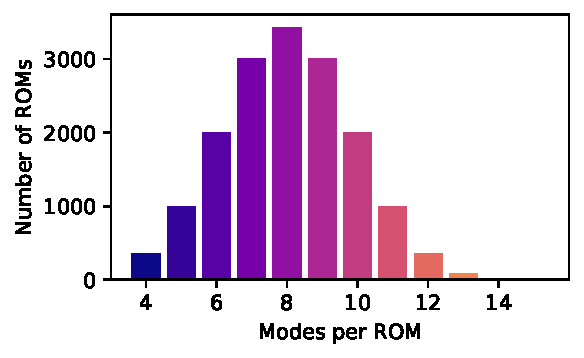
\includegraphics[width=0.5\linewidth]{figs/caseCounts_20240828.pdf}
    \caption{l number of mode combinations used to reconstruct the flow field for a given maximum number of modes considered ($k$). For all cases, only modes 1 through 15 are considered ($N_r=14$).}
    \label{fig:caseCounts_20240828}
\end{figure}

For each ROM, velocity fields are reconstruction from the truncated basis, summing over selected mode indices, rather than a sequential set up to a maximum. 
For each combination $I=\binom{N}{k}$, the reconstructed velocity field is,
\begin{equation}
  \hat{u}(\bm{x},t) = \sum_{i \in I} a_i(t) \Phi^{(i)} (\bm{x})
  \label{eq:PODset}
\end{equation}
where the index $i$ may take only the values included in a particular combination of modes and the hat notation indicates a low-dimensional representation of the velocity field. 
In \cref{eq:PODset}, the velocity field and modal basis have been denoted as scalars, as only the streamwise component of velocity is considered. 
%The scanning lidar returns only the line-of-sight velocity, which is converted into the streamwise velocity, but does not include other velocity vector components.

%%%%%%%%%%%%%%%%%%%
\section{Data} % (fold)
\label{sec:Data}

This work makes use of nacelle-mounted scanning lidar data and atmospheric inflow measurements from two recent DOE-funded field campaigns.
The American WAKE ExperimeNt (AWAKEN\cite{moriarty2024overview}) is a multi-institutional field campaign designed to gather critical data on wind farm-atmosphere interactions, which contribute to uncertainty in wind plant performance models. 
% Data collected in the AWAKEN project are intended to help support model development and validation, ultimately reducing uncertainty and increasing wind energy profitability. 
% Observations from 13 ground-based locations and five wind turbines in Northern Oklahoma will be made publicly available to advance wind energy science and improve system reliability.
% Within the scope of this work, data sets from several sources in the AWAKEN Project have been considered.
Atmospheric conditions were characterized through a combination of metrics derived from a surface flux station \cite{a2e_awaken_surfaceMet} and a meteorological tower \cite{a2e_awaken_kS_metTower} located at site A1. 
The surface flux station features a Gill R3-50 sonic anemometer mounted on a 4-meter-high tripod, recording data continuously at a 20 Hz rate. 
Data acquisition used software originally developed by Argonne National Laboratory for the ARM ECOR system in 2003, which was adapted for the AWAKEN project to work with Gill Sonic R3 series anemometers.\cite{cook2018eddy} 
Sensible heat flux and momentum flux were processed into data at 30 minute resolution, assuming a constant relative humidity of 50\% due to the absence of real-time humidity measurements. 
Hub-height wind speed and wind direction were recorded with a Thies 3D Ultrasonic anemometer. Turbulence intensity was estimated as a 10-min rolling calculation of the standard deviation of wind speed divided by mean wind speed in the same period.
Wind directions were limited to a sector ranging from 170$^\circ$ to 200$^\circ$, corresponding to the peak of the wind rose shown in \cref{fig:awakenSchem}. 
This also limited times when the wake from a neighboring turbine were visible in the data.

\begin{figure}[htbp]
  \centering
  \begin{subfigure}[b]{0.6\columnwidth}
    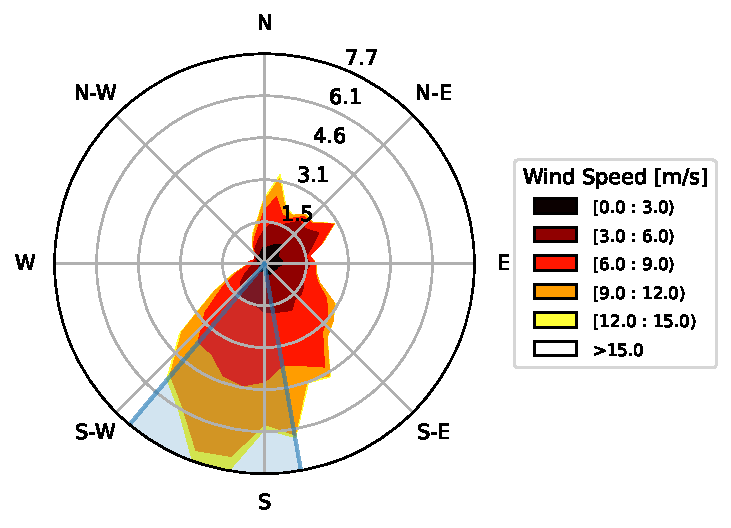
\includegraphics[width=\columnwidth]{figs/windrose_20240828.pdf}
  \end{subfigure}
  \begin{subfigure}[b]{0.38\columnwidth}
    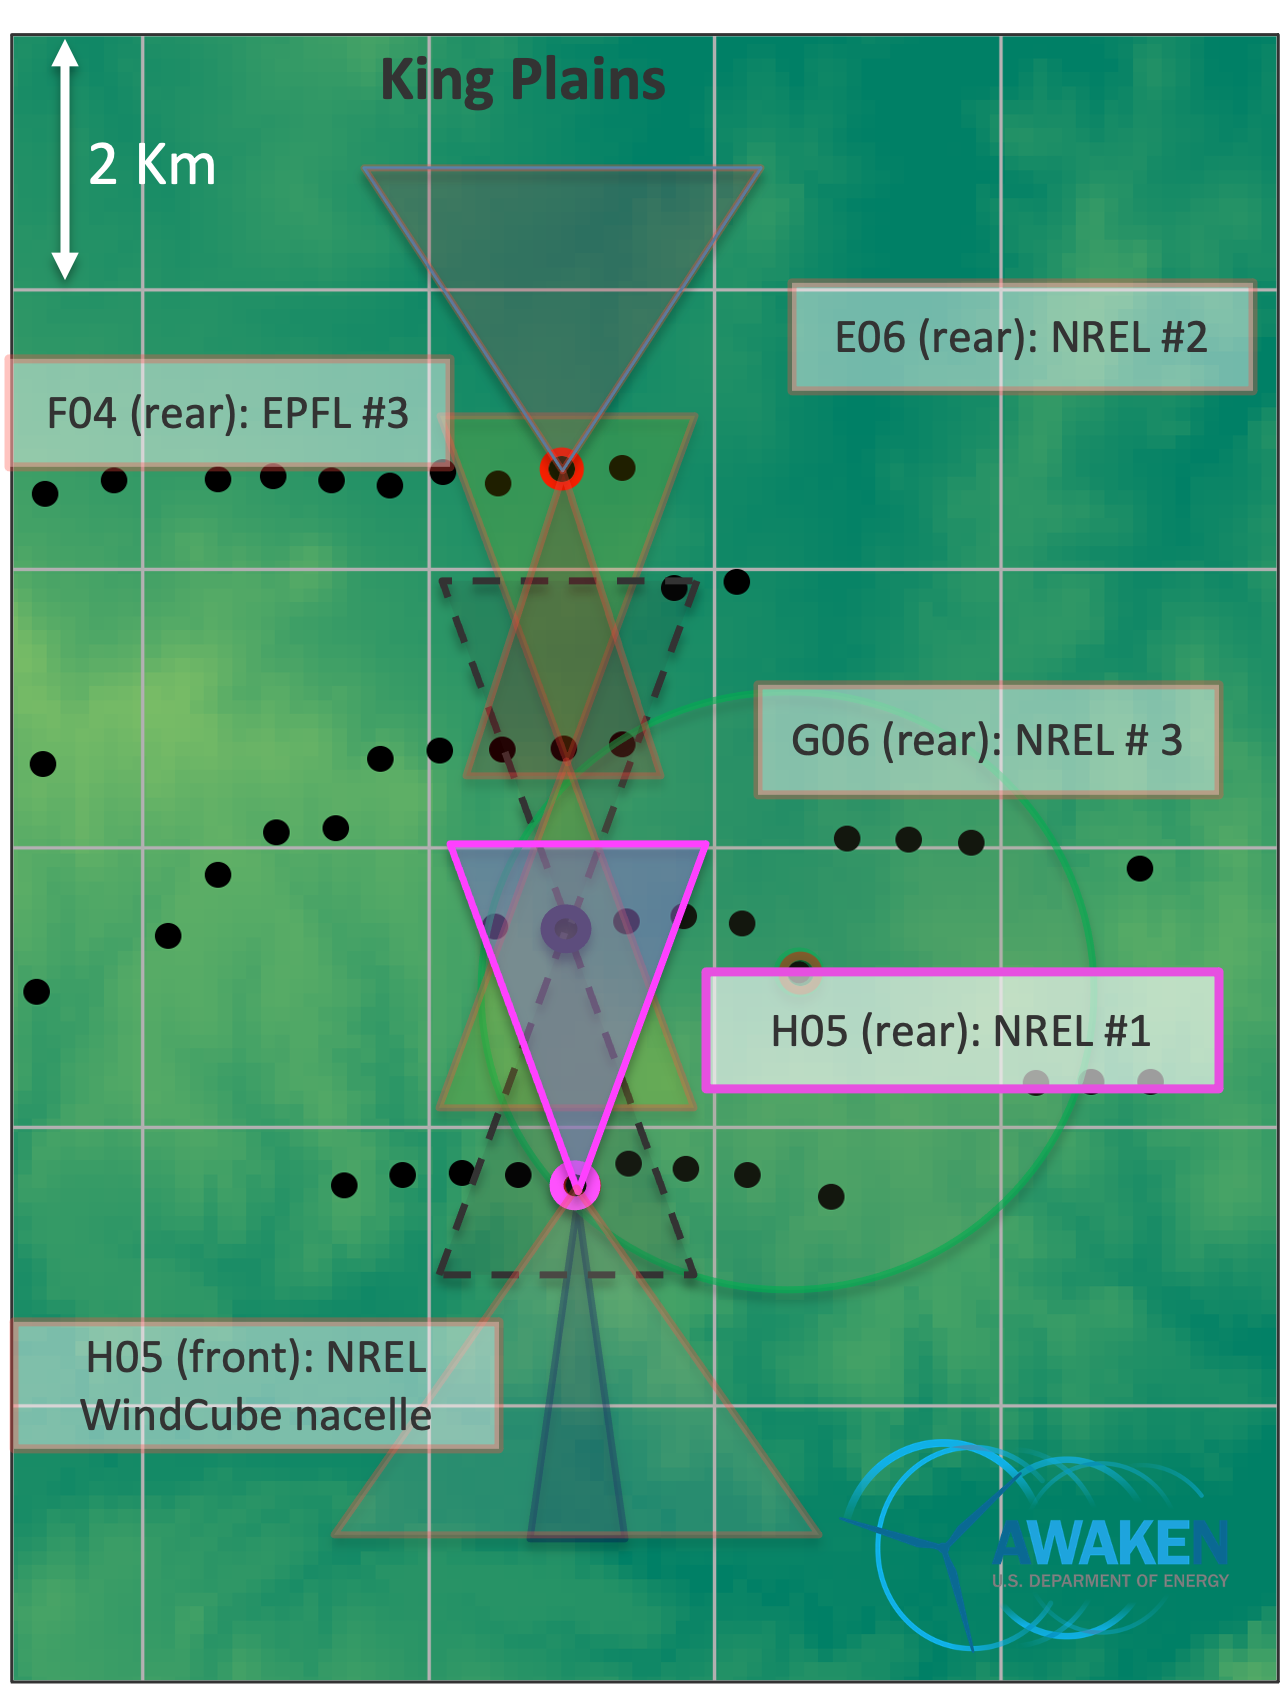
\includegraphics[width=\columnwidth]{figs/20240923.AWAKEN.awakenSchem.png}
  \end{subfigure}
  \caption{Wind rose showing selected wind direction sector in blue (left) and high-level schematic (right) of the AWAKEN project.}
  \label{fig:awakenSchem}
\end{figure}


\begin{figure}[htbp]
  \centering
  \begin{subfigure}[b]{0.6\columnwidth}
    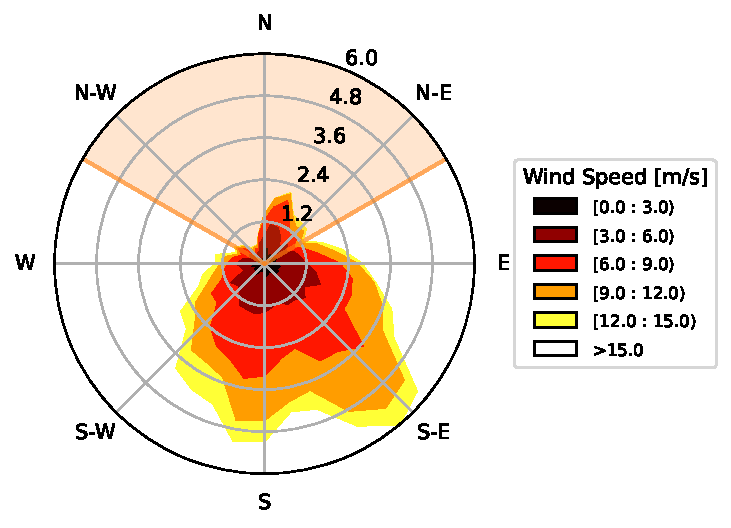
\includegraphics[width=\columnwidth]{figs/20241206.RAAW.windrose.pdf}
  \end{subfigure}
  \begin{subfigure}[b]{0.3\columnwidth}
    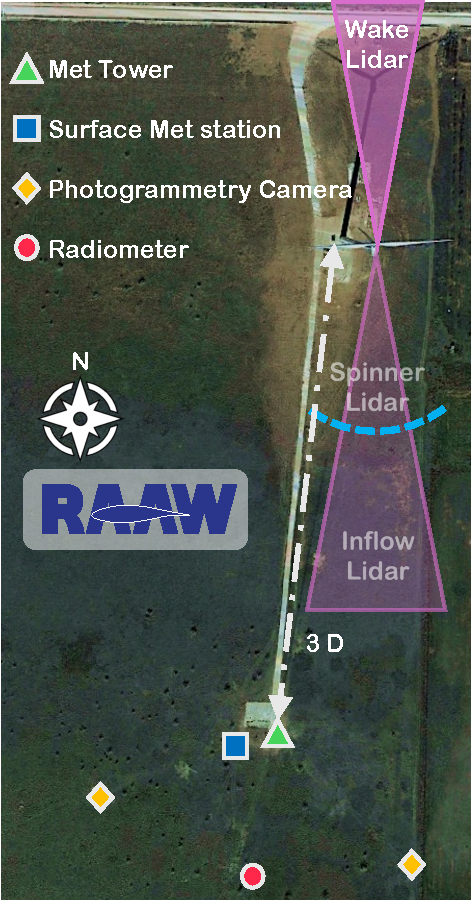
\includegraphics[width=\columnwidth]{figs/20241206.RAAW.schem.pdf}
  \end{subfigure}
  \caption{Wind rose showing excluded wind direction sector in orange (left) and high-level schematic (right) of the RAAW project.}
  \label{fig:raawSchem}
\end{figure}


% \item[nacelle-mounted lidar observations] are used to quantify momentum deficits, flow features, and wake meandering 

The Rotor Aerodynamics, Aeroelastics, and Wake (RAAW) project is a field campaign designed to study the performance of modern flexible rotor wind turbines. 
Atmospheric inflow conditions for data cases in the RAAW project are derived from a 183.5-meter guyed meteorological tower, instrumented between the rotor bottom and top heights with 5 cup anemometers, 3 ultrasonic anemometers, 3 vanes, 3 barometric and temperature sensors, and one humidity sensor.
Ultrasonic anemometers reported data at 20 Hz, and all other instruments at 1 Hz.
Near-surface measurements of momentum and heat flux were provided by a surface met station, deployed approximately 10 meters southwest of the meteorological tower, that hosted an ultrasonic anemometer measuring at 2.5 m above ground and a probe for atmospheric pressure, temperature and humidity 2 m above ground. 
Similarly to the tall tower sensors, the anemometer reported data at 20 Hz and the other sensors at 1 Hz.
\comment{Figure XXX} shows the experimental arrangement of the RAAW project, including the met tower, surface met station, and turbine.
\comment{NEED A RAAW CITATION, when will the report be done?}

% \begin{figure}[h]
%     \centering
%     \includegraphics[width=0.5\linewidth]{figs/raa.png}
%     \caption{ high-level schematic (right) of the RAAW project showing the wind turbine, met tower, and associated instrumentation.}
%     \label{fig:raawSchem}
% \end{figure}



Both the RAAW and the AWAKEN project feature GE 2.8 MW turbines with 127 m rotor diameters. The RAAW project made use of a prototype R\&D turbine located in Lubbock, TX, that had a hub height of 120 m. 
In the AWAKEN project, the turbines are production-run GE2.8-127 turbines with a hub height of 88.5 m. 
% \cref{fig:turbine_photo}. 
In both projects, Halo Photonics Streamline XR+ Doppler scanning lidars were positioned on the aft sections of the nacelles of the turbines of both projects and were configured for a variety of measurement strategies, including a plan-position indicator (PPI) scan optimized to measure the flucutating flow fields in the wake.
Wake PPIs were designed using the LiSBOA tool \cite{letizia2021lisboa}, sweeping approimately 1$^\circ$ of azimuth per second convering a sector of approximately 20$^\circ$ centered downstream of the turbine.
Lidar data were quality controlled using the FIeld EXperiments Tool Arsenal (FIEXTA) software \cite{nrelfiexta2024} that includes the dynamic filtering methods outlined by \citet{beckDynamicDataFiltering2017}.
Data are temporally upsampled considering local advection velocities and the time delays between successive beams at similar azimuth angles,\cite{beckTemporalUpSamplingPlanar2019} producing line-of-sight velocity `snapshots' at a temporal resolution of 1 second.
% Line of sight velocity is used in the subsequent analysis without transformation into Cartesian velocity vector components.
% The analysis in this work uses data from a single scanning lidar only, performing a sector scan at hub height with a range gate of 18 m and an angular resolution of 2$^\circ$. Each sector scan took approximately 7 sec to complete. As the lidar was fixed to the nacelle, the center line of the nacelle is represented as zero azimuth for the lidar scans, and the lidar scan covered $\pm14^\circ$ from the center line.
Scanning lidar provides line-of-sight wind speed, $v_{los}$. The horizontal wind speed, $u$ was retrieved as,
\begin{equation}
v_\text{los}(r)=u \cos\zeta \cos(\psi-\theta)+ w\sin\zeta
\label{los wind speed}
\end{equation}
where $u$ is the horizontal wind speed, $r$ represents the range along the laser beam, $\zeta$ is the elevation angle, $\psi$ is the azimuth angle, and $\theta$, is the wind direction. 
% The wind direction, $\theta_o$, is estimated based on the nacelle position and wind direction measured by a nacelle-mounted wind vane \cite{Simley2020}. 
For all lidar measurements used in the following analysis, the elevation angle was fixed at 0$^\circ$, simplifying the relationship between $v_\text{los}$ and $u$.

% The full analysis we undertake in the current work seeks wake center locations in the quality-controlled scanning lidar data described above. 
While the lidars are capable of making measurements up to 4 km from the wind turbine, the measurement qualilty is typically quite low, and wakes are often fully recovered far sooner.
Additionally, the data collected in the AWAKEN project include only inflows from a southerly sector, and the downstream row of turbines is often visible in the scan data. 
To preclude observations of wakes of neighboring turbines from influencing wake center estimates, which would complicate the modal analysis undertaken below, scans are constrained to ranges where $2.5 \le x/D \le 10$ and azimuth angles $-20^\circ \le \alpha \le 20^\circ$.
\comment{check azimuth limits}

Each data set of continuous PPI scans lasted approximately 30 minute, with a full azimuthal sweep occuring approximately every 18 to 20 seconds.
After spatiotemporal upsampling following the procedure outlined in \citet{beckTemporalUpSamplingPlanar2019}, each data case from the AWAKEN project contained approximately 1,650 snapshots (complete, infilled scans) at temporal resolution of 1 s. 
Data cases from the RAAW project are contained in 15 minute sections, leading to upsampled and infilled data sets of approximately 800 scans each at a temporal resolution of 1 s.

% filter metrics
% np.round((100*(1-qcdf.astype(int).sum(axis=0)/len(qcdf))),2)
% filterStuckSensor     0.00
% filterYawTravel      51.25
% filterActivePower    18.50
% filterTVar           10.03
Measurement cases combining lidar data sets and inflow measurements were considered only after passing through the following quality control filters. Each filter is followed by a metric indcating the portion of the population of data that were disallowed and a description. Note that more than one filter condition was applicable to many of the data points.
\begin{description}
  \item[Sensor Quality---6\%] Measurement cases combining lidar data sets and inflow measurements were considered only after filtering out stuck, broken, or defective sensors. This ensures that all required measurements are reliable and eliminates cases where data are missing or sensors fail to report reasonable observations.
  \item[Wind Direction Sector---34\%] Cases were filtered to include only wind directions within the appropriate sector. This is crucial because we rely on the characteristics of the inflow to contextualize wind turbine wake meandering. For the AWAKEN project, this step also ensures that only the wake dynamics from the single turbine of interest are present in the lidar scans.
  \item[Yaw Travel Limitation---51\%] Only cases with a total yaw travel below 20$^\circ$ were considered. In both the RAAW and AWAKEN projects, the wind turbine operates at a nominal control point, allowing the rotor to yaw and optimally align with the incoming wind. Yaw activity is evident in lidar scans as abrupt changes or sweeping movements of the wakes within the scanned sectors. Very few lidar scan periods are completely free from yaw activity, hence the 20$^\circ$ travel limitation.
  \item[Power Production Threshold---18\%] Cases were filtered to include only those where active power is greater than 150 kW. This criterion ensures that the turbine is operating within region 2 of the power curve and that a wake will be evident in the lidar data. The selection allows for describing wake meandering under a wide range of atmospheric conditions and inflow wind speeds.
  \item[Variability Filtering---10\%] As a final quality control step, cases were excluded where the total variation exceeded the 90\textsuperscript{th} percentile. Following the method outlined by Hamilton,\cite{hamilton2020atmospheric} total variation is defined as the determinate of the covariance matrix relating inflow wind speed, wind direction, turbulence intensity, turbine power production, and nacelle position signals from the SCADA record. This step ensures that only statistically stationary conditions are considered, eliminating cases with drastically changing atmospheric conditions or significant turbine control actions during the lidar scan period.
\end{description}
A total of 65 cases were retained after applying each of the quality control filters enumated above, including 54 cases from the AWAKEN proejct and 11 cases from the RAAW project.
\Cref{fig:power_curve_cases} shows the distribution of the full range of cases with wake PPI scans. 
Cases that did not pass all of the quality control measures listed above are shown in gray. 
The final cases selected for analysis are highlighted in the figure according to the total yaw travel observed during the respective wake scanning period.
\begin{figure}
    \centering
    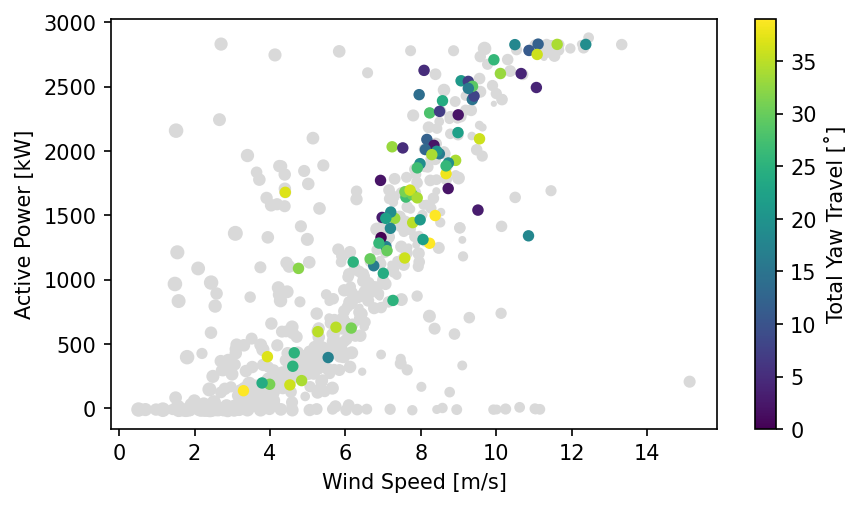
\includegraphics[width=0.65\linewidth]{figs/20240911.AWAKEN.power.curve.cases.png}
    \caption{Power curve from turbine H05 at the King Plains Wind Plant. All available cases are shown with gray points, cases selected for analysis in the current work are colored by the total yaw travel of the turbine during the measurement period.}
    \label{fig:power_curve_cases}
\end{figure}

The integral time scale of atmospheric turbulence provides a measure of the temporal correlation of velocity fluctuations in the atmospheric boundary layer. 
The autocorrelation coefficient $\rho(\tau)$ is then defined as:
\begin{equation}
\rho(\tau) = \frac{\langle u'(t)u'(t+\tau) \rangle}{\sigma^2}
\end{equation}
where $u'(t)$ represents the turbulent velocity fluctuations, $\tau$ is the time lag, $\langle \cdot \rangle$ denotes the ensemble average, and $\sigma^2$ is the variance of the velocity fluctuations.
The integral time scale $T$ is calculated by integrating the autocorrelation function up to the point where it decays to a specified threshold:
\begin{equation}
T = \int_{0}^{\tau_c} \rho(\tau) , d\tau
\end{equation}
Here, $\tau_c$ represents the correlation decay limit, typically chosen as the point where $\rho(\tau) = 0.05$, rather than the first zero-crossing point.\cite{Simley2015, Debnath2020}
This integration captures the temporal coherence of turbulent fluctuations, providing insight into the characteristic time scales of atmospheric turbulence.
In practice, this calculation was performed using 20-Hz wind speed measurements from a sonic anemometer positioned at hub height for the turbines in each project, with computations based on 30-minute averaging periods. 


\Cref{fig:ts} shows the distribution of inflow wind speed, $U_\infty$, integral time scale, $T$, and inflow Strouhal number, $St_\text{in}$ for each of the 71 cases from the combined RAAW aand AWAKEN experiments.
The integral time scales, $T$, are taken as the characteristic period of the fluctuation in the velocity field and are used to define the characteristic frequency of turbulent fluctuations in the discussion of meandering frequencies. 

\begin{figure}[h]
  \centering
  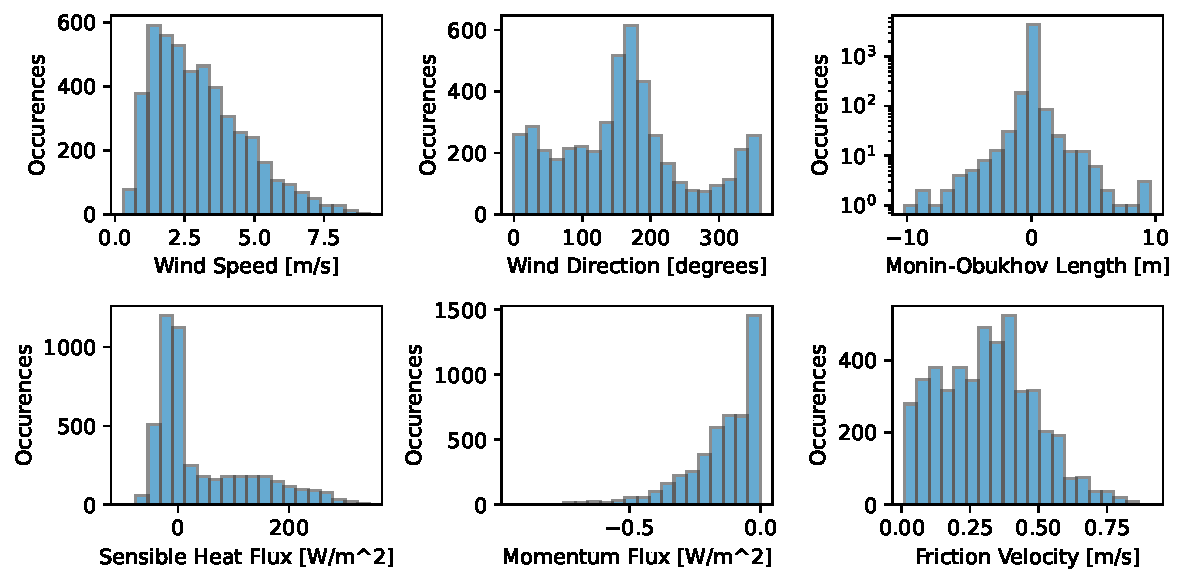
\includegraphics[width=\textwidth]{figs/20241205.inflowStats.pdf}
  \caption{Distributions of the average inflow conditions observed at the surface met stations at Site A1 throughout the AWAKEN and RAAW campaigns.}
  \label{fig:inflowStats}
\end{figure}

\begin{figure}[h]
    \centering
    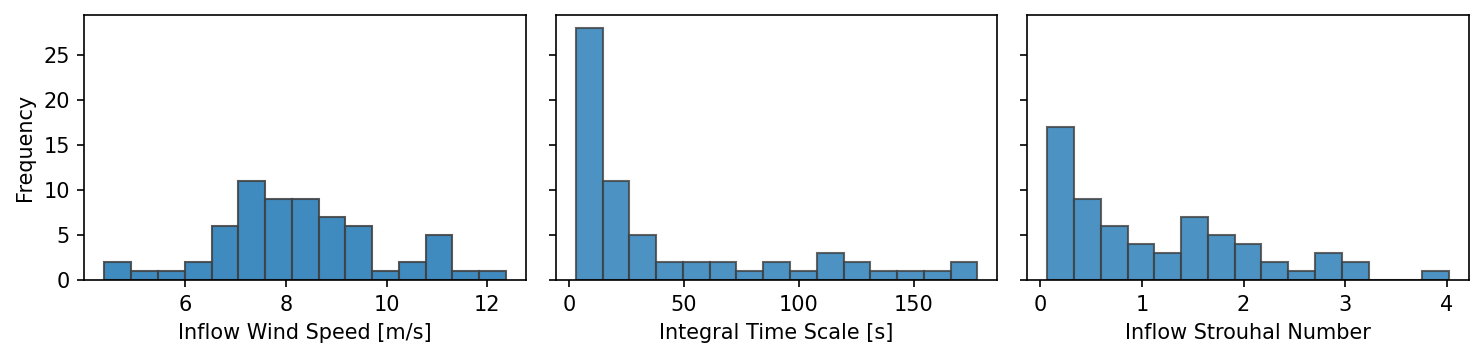
\includegraphics[width=\textwidth]{figs/20240924.AWAKEN.inflow.WS.TS.ST.png}
    \caption{Distributions of the average inflow wind speed, $U_\infty$, integral time scale, $T$, and Strouhal Number, $St_\text{in}$, at hub height for the subset of conditions corresponding to the 65 selected cases.}
    \label{fig:ts}
\end{figure}

%%%%%%%%%%%%%%%%%%%%%%%%%%
\section{Results} % (fold)
\label{sec:Results}
%%%%%%%%%%%%%%%%%%%%%%%%%%

Average scans shown for selected cases are shown in \cref{fig:aveScans} and highlight differences in the peak momentum deficit and recovery rate of wakes in different atmospheric conditions.
While all data sets include some yaw activity, the average wake is centered around $\alpha=0$. 
Each of time-averaged velocity fields in \cref{fig:aveScans} highlights characteristics of the wind turbine wake as well as the influence of the atmsopheric forcing conditions and effects of the wind turbine operations and controls. 
The data quality control preferntially selecetd the most statistically stationary cases from the full population of data.
As a consequence of this selection, there is a bias toward stable atmospheric conditions in which the yaw travel was minimized during the lidar collection periods of both experiments.

\begin{figure}[htbp]
  \centering
  \begin{subfigure}[b]{0.48\columnwidth}
    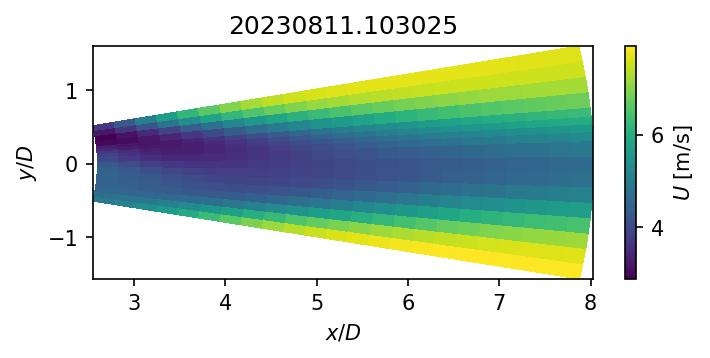
\includegraphics[width=\columnwidth]{figs/U.lidar.20230811.103025.png}
  \end{subfigure}
  \begin{subfigure}[b]{0.48\columnwidth}
    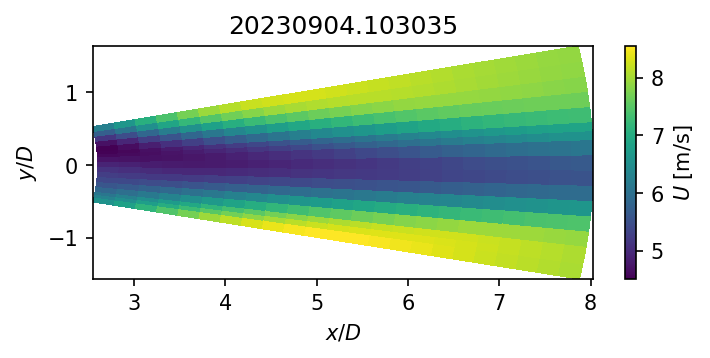
\includegraphics[width=\columnwidth]{figs/U.lidar.20230904.103035.png}
  \end{subfigure}

  \begin{subfigure}[b]{0.48\columnwidth}
    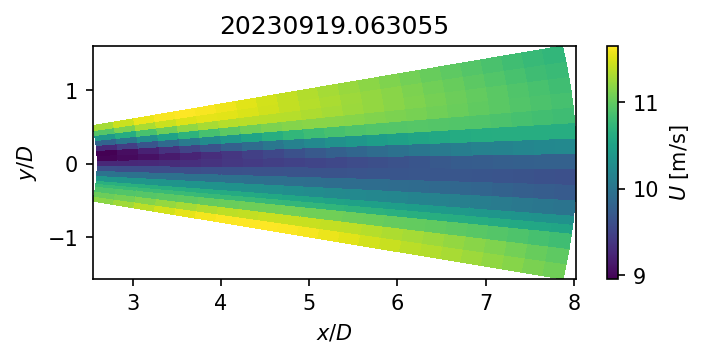
\includegraphics[width=\columnwidth]{figs/U.lidar.20230919.063055.png}
  \end{subfigure}
  \begin{subfigure}[b]{0.48\columnwidth}
    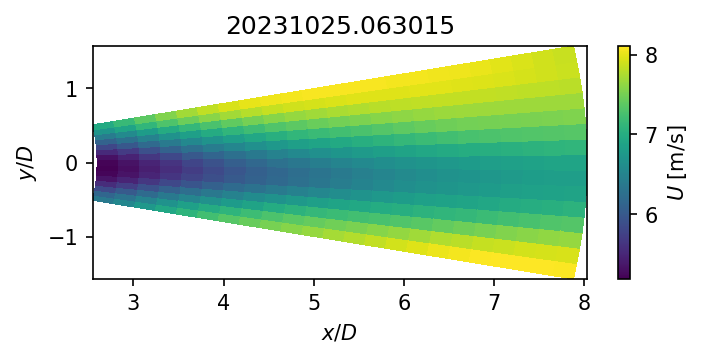
\includegraphics[width=\columnwidth]{figs/U.lidar.20231025.063015.png}
  \end{subfigure}
  \caption{Average wake velocity fields for 2023-08-11 10:30 (top left),
  2023-09-04 10:30 (top right),
  2023-09-19 06:30 (bottom left),
  2023-10-25 06:30 (bottom right) showing a range of background velocities, momentum deficits and wake recovery rates.}
  \label{fig:aveScans}
\end{figure}


\begin{figure}[htbp]
  \centering
  \begin{subfigure}[b]{0.48\columnwidth}
    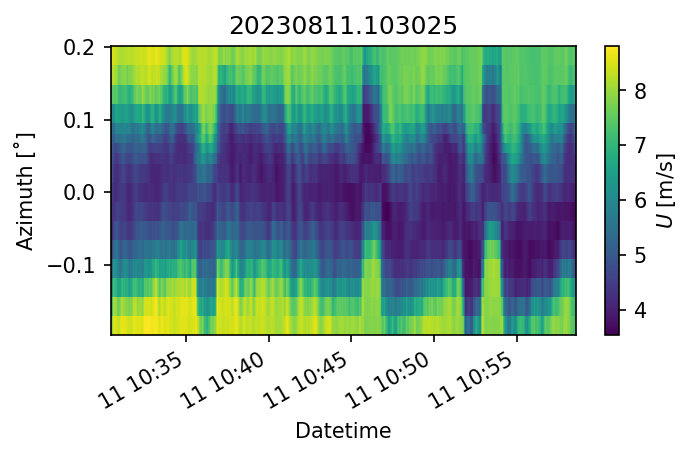
\includegraphics[width=\columnwidth]{figs/crossSection.lidar.20230811.103025.png}
  \end{subfigure}
  \begin{subfigure}[b]{0.48\columnwidth}
    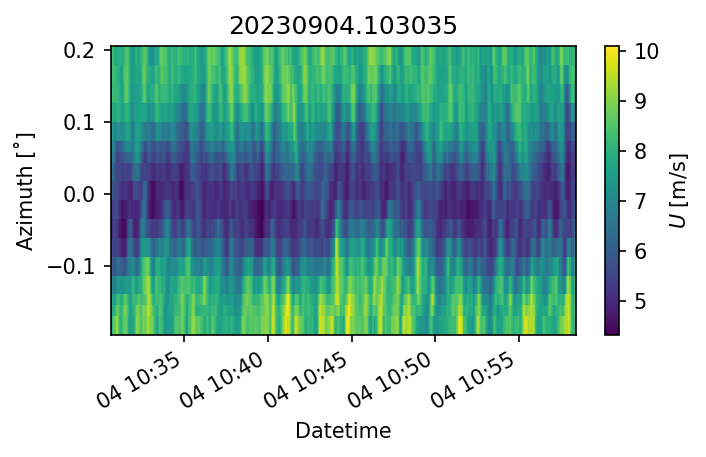
\includegraphics[width=\columnwidth]{figs/crossSection.lidar.20230904.103035.png}
  \end{subfigure}

  \begin{subfigure}[b]{0.48\columnwidth}
    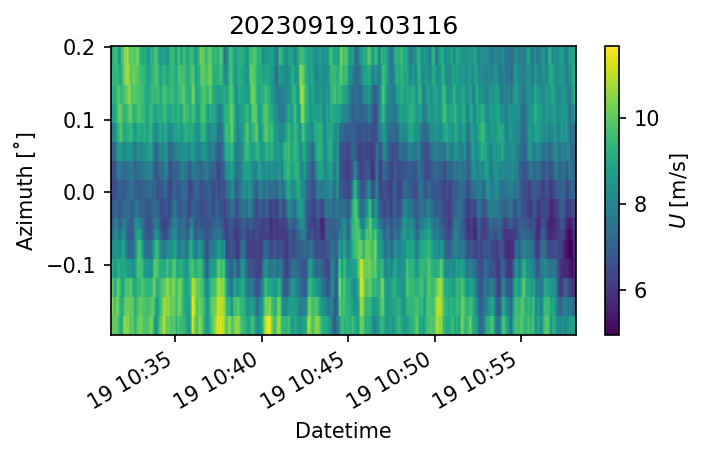
\includegraphics[width=\columnwidth]{figs/crossSection.lidar.20230919.103116.png}
  \end{subfigure}
  \begin{subfigure}[b]{0.48\columnwidth}
    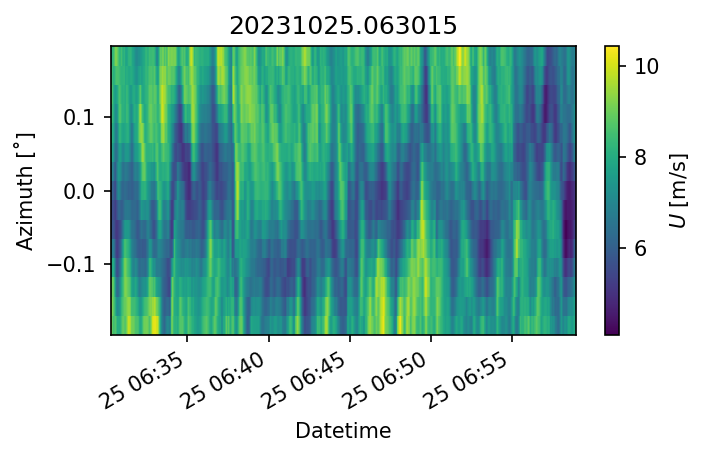
\includegraphics[width=\columnwidth]{figs/crossSection.lidar.20231025.063015.png}
  \end{subfigure}
  \caption{Average wake velocity fields for 2023-08-11 10:30 (top left),
  2023-09-04 10:30 (top right),
  2023-09-19 06:30 (bottom left),
  2023-10-25 06:30 (bottom right) showing a range of background velocities, momentum deficits and wake recovery rates. }
  \label{fig:crossSection}
\end{figure}

\begin{figure}[h]
  \centering
  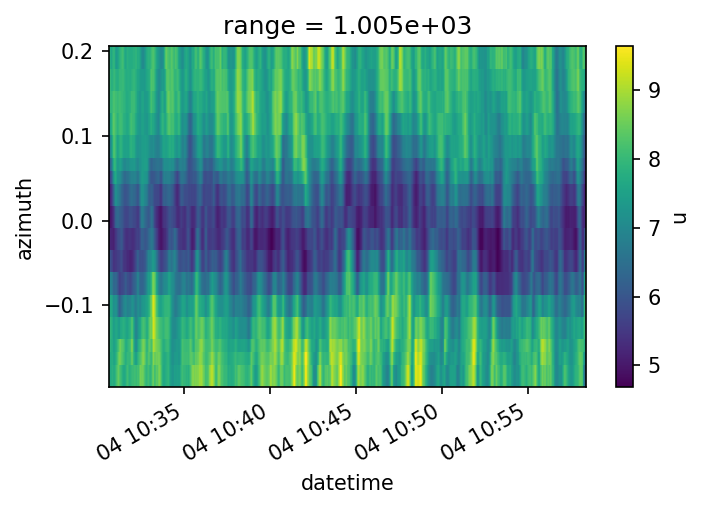
\includegraphics[width=0.5\textwidth]{figs/20230904.AWAKEN.lidarX103004.png}
  \caption{Time-azimuth cross section of a line of sight velcoity from a lidar scan at 8$D$ downstream of the lidar. The wake is shown in dark blue and background velocity in green/yellow. }
  \label{fig:lidarAzTime}
\end{figure}


Yaw activity is not directly evident in the time-averaged wakes.
However, \cref{fig:crossSection} shows a time-azimuth cross section of a single dataset at a range of approximately $x/D=8$ (1 km), in which the wake is highlighted as a low wind speed region that persists in time across the figure.
Meander in the azimuthal direction seen in the figure combines the effects of several factors. 
While the wake center does travel horizontally, there are also translations of the wake center introduced by the yaw activity of the rotor.
Horizontal wake center locations, $\mu$ are estimated as the center loaction of the Gaussian function fit to the velocity deficit, as in \cref{eq:gaussfit}.
Yaw activity becomes especially evident in the time histories of detected wake centers, presented in \cref{fig:yawCorrectedWakeCenter}.
Yaw activity, illustrated by the dashed black line and related vertical axis on the right, are evident in the detected centers as sudden shifts in the wake center time histories. 
Because changes in the nacelle position impact the apparent wake centers uniformly at all ranges, a simple correction can be applied to the wake centers as, $\Delta \mu = r \sin{\psi}$,
% \begin{equation}
%   \Delta \mu = r \cos{\psi}
% \label{eq:deltamu}
% \end{equation}
where $r$ indicates the distance from the lidar (range) and $\psi$ indicates the nacelle orientation with respect to the position at the beginning of each data set. 
Correcting for changes in nacelle position throughout each dataset is important to correctly characterize the distributions of wake centers and their dynamics in the turbine frame of reference.
% TODO: add to discussion
It should be noted that turbines take yaw-correcting actions only after after an integrator of error between the measured wind direction and the nacelle position exceeds a threshold.
This means that in most cases there remains some influence of yaw misalignemnt on the detected wake centers even after correcting for yaw activity. 
Without a time history, it is not possible to accurately account for the yaw error.
However, this sort of misalignment is part of the nominal operation of a turbine under normal control conditions, and is a possible trigger for wake meandering.

\begin{figure}[h]
  \centering
  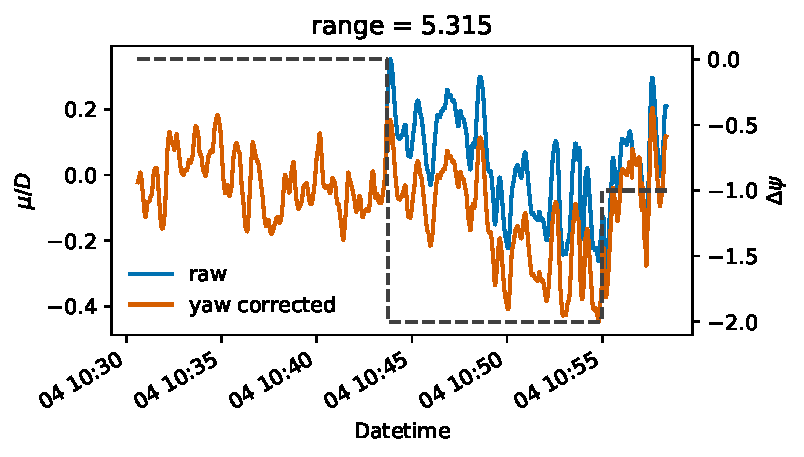
\includegraphics[width=0.5\textwidth]{figs/yawCorrectedWakeCenter_20240925.pdf}
  \caption{Detected wake centers directly from lidar observations (blue) and after correcting for yaw activity of the turbine (orange). The dashed black line indicates nacelle position changes from the beginning of the time series and corresponds with the axis labels on the right.}
  \label{fig:yawCorrectedWakeCenter}
\end{figure}

An example of the momentum deficit measured by the lidar is shown in \Cref{fig:wakeCenterByRange} in blue, along with local fits of the Gaussian function in black and detected wake centers as red points. 
Each of the subfigures indicate a good level of agreement between the momentum deficit and fit function, building confidence in the Gaussian model of the wake.
Alternative methods of detecting the wake centers have been explored in the literature,\cite{brugger2020lidar} including a momentum-centroid approach and local minimum velocity methods, but are not explored in the current work for brevity.
\begin{figure}[h]
  \centering
  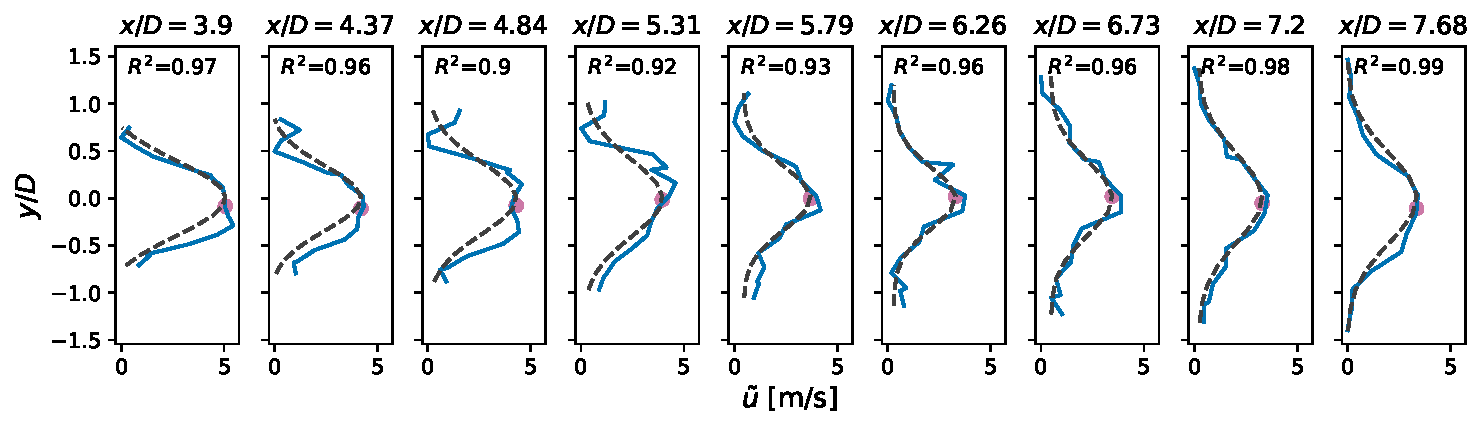
\includegraphics[width=\textwidth]{figs/wakeCenter_byRange_20240927.pdf}
  \caption{Detected wake centers showing Guassian fit against momentum deficit. Blue lines indicate momentum deficit estimated from lidar scans, dashed line shows the fit Gaussian profile, point marker is is the detected wake center $\mu/D$. \comment{add $R^2$ value to each supblot}}
  \label{fig:wakeCenterByRange}
\end{figure}

An alternative view of the detected wake centers is provided in \cref{fig:lidarScanCenters}, where $\mu/D$ is noted on the lidar scans as points colored by their respective $R^2$ values. 
In both examples, it is evident that the $\mu/D$ follows the bluk momentum deficit in the wake quite closely.
A bias of $\mu/D$ toward positive values of $y/D$ in the near wake $x/D \lesssim 3$ is also visible in the scan taken at 2023-09-04 10:42:15 UTC (left).
This bias, which persists throughout many of the scans, arises from the asymmetric double-Gaussian profile of the momentum deficit very near the turbine.\cite{schreiber2020brief,keane2021advancement,sadek2023three}
Positive bias of $\mu/D$ in the near wake is not easily corrected, and leads to impacts later in the analysis, including power spectral densities an representation with the ROMs. 

\begin{figure}[htbp]
  \centering
  \begin{subfigure}[b]{0.49\columnwidth}
    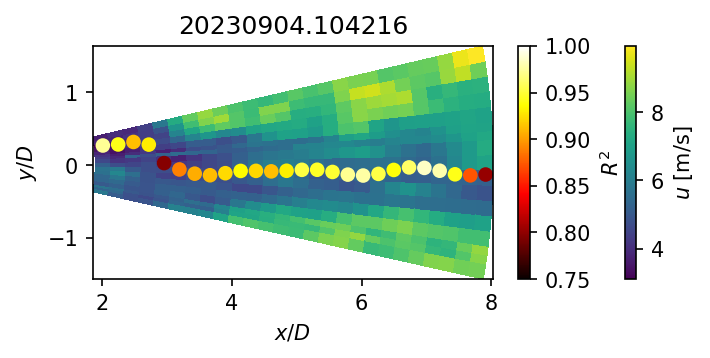
\includegraphics[width=\columnwidth]{figs/lidarScan_700_wakeCenters_20240925.png}
  \end{subfigure}
  \begin{subfigure}[b]{0.49\columnwidth}
    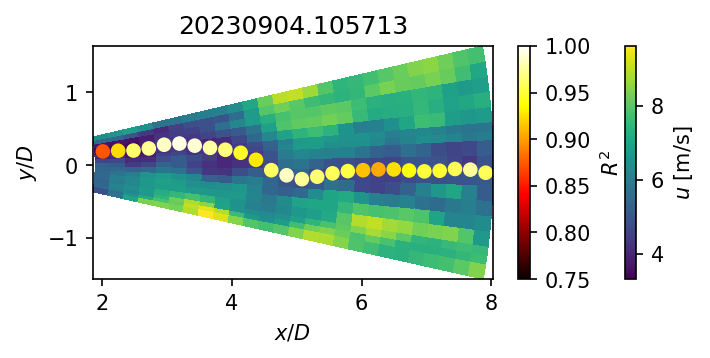
\includegraphics[width=\columnwidth]{figs/lidarScan_-70_wakeCenters_20240925.png}
  \end{subfigure}  
  \caption{Example lidar scans showing $u$ overlaid with the fitted wake centers. Detected wake centers are colored by their respective coefficent of determination.}
  \label{fig:lidarScanCenters}
\end{figure}

Wake meandering combines the downstream advection of $\mu$ by the mean flow and turbulent structures in the wake.
Trajectories of $\mu$ throuhgout the measurement domain are shown in \cref{fig:centerDistributions} (left) for several times in the data set.
The trajectories all show the positive bias of $\mu$ in the near wake and then tend toward negative values of $y$ as the range (downstream distance) increases.
The meander is also evident in the trajectories as a local tendency back toward positive values of $y$.
The amplitdues of these meandering structures also tend to increase as they advect downstream.
Kernel density estimates of wake center locations are shown in \cref{fig:centerDistributions} (right), highlighting the tendency of the $\mu$ to spread out at greater streamwise distances.

\begin{figure}[htbp]
  \centering
  \begin{subfigure}[b]{0.57\columnwidth}
    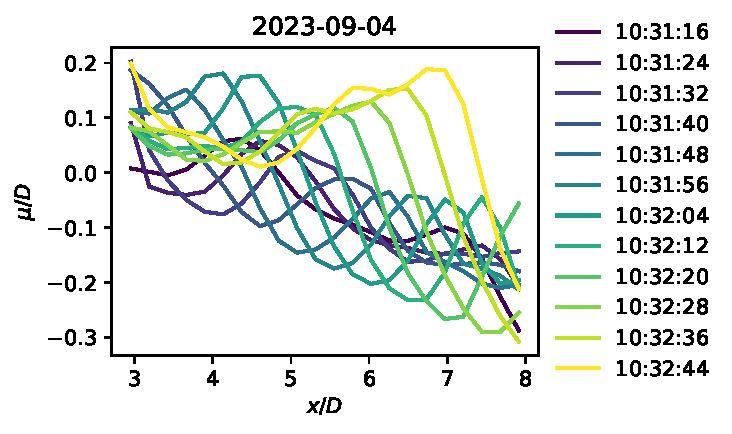
\includegraphics[width=\columnwidth]{figs/wake_center_advection_20240925.pdf}
  \end{subfigure}
  \begin{subfigure}[b]{0.42\columnwidth}
    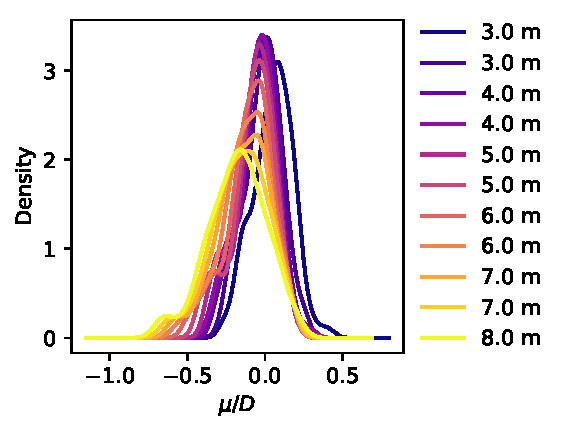
\includegraphics[width=\columnwidth]{figs/wake_center_kde_20240925.pdf}
  \end{subfigure}
  \caption{Wake center trajectories for selected times (left) and kernal density estiamtes of wake centers by distance downstream of the lidar (right).}
  \label{fig:centerDistributions}
\end{figure}

In addition to statistical descriptions of the wake center, we are also interested in dynamics of wake meandering, specifically relating the characteristic frequencies of wake meandering, quantified through power spectral densities (PSD, \cref{eq:psd}) to inflow conditions and the POD modes, $\phi_i$.
PSDs are calculated using Welch's method as,
\begin{equation}
  S_{\mu\mu}(f) = \frac{1}{L} \sum_{k=1}^{K} \frac{1}{N} \left| \sum_{n=1}^{N} \mu_k(n)  e^{-i 2\pi f n / N} \right|^2  
\label{eq:psd}
\end{equation}
where, $K$ is the number of segments,
$L=512$ samples is the number of points in the FFT
$N=1,024$ is the length of each segment,
$\mu_k(n)$ is the $k$-th segment of the time series. 
A uniform window function is applied to each segment in the calculation of the PSDs.
The frequency range for all spectra in the current work have been normalized with the average inflow velocity recorded by the met towers, $U_\infty$, and the turbine's rotor diameter, $D$, as $f_{St} = f * D / U_\infty$

\begin{figure}[htbp]
  \centering
  \begin{subfigure}[b]{0.48\columnwidth}
    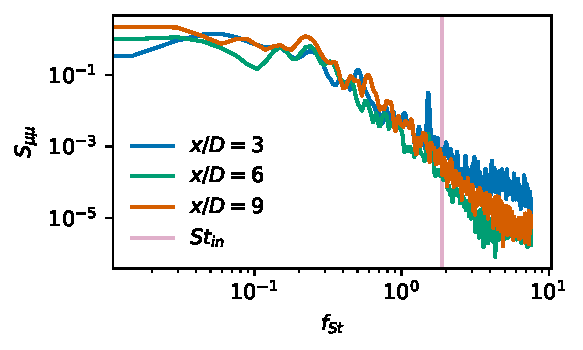
\includegraphics[width=\columnwidth]{figs/wake_center_spectra_20240927.pdf}
  \end{subfigure}
  \begin{subfigure}[b]{0.48\columnwidth}
    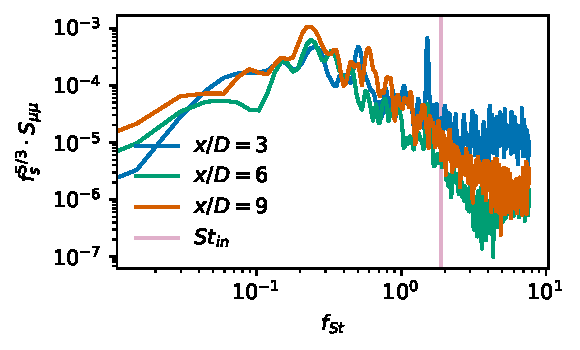
\includegraphics[width=\columnwidth]{figs/wake_center_premult_20240927.pdf}
  \end{subfigure}
  \caption{PSDs (left) and premultiplied spectra (right) of detected wake centers from the lidar data at selected downstream distances. \comment{fix vertical axis label for premult spectra}}
  \label{fig:lidarSpec}
\end{figure}



% ### POD
The snapshot POD introduced in Section \ref{sec:POD} requires state space observations with consistent dimensions and coordinates, making it impractical to correct for yaw before decomposition. 
Remapping wake observations from lidar scans onto a corrected reference frame downstream of the turbine would introduce inconsistencies in the azimuthal coordinates or create empty radial slices, both of which would complicate the eigenvalue decomposition central to the POD analysis.

Each of the 74 cases analyzed here has slightly varying azimuth coordinates due to the continuous scan operation of the lidar, which assigns nominal azimuth angles after a set time delta. 
Small variations in the number of scans per dataset arose from operational delays, data transmission, and status checks.
Here, we focus on the low-rank POD modes, which account for the bulk of the turbulent kinetic energy (TKE) in the lidar scans.
Although the energy distribution across POD modes differs for each dataset, the modes are ordered by descending energy, with the eigenvalue $\lambda_i$ of each mode representing the energy distribution.

Only the first 14 POD modes, which contain the most coherent structures in the lidar scans, are used in flow field reconstructions for meandering analysis. The eigenvalues $\lambda_i$ also quantify the TKE captured in each reduced-order model (ROM), providing a direct measure of reconstruction error. Missing energy in a ROM is bounded by the smallest mode eigenvalue included in the reconstruction. \Cref{fig:cumLamNorm} shows the distribution of TKE described by the POD modes across all cases. 
The energy of the zeroth mode $\phi_0$, which represents the mean flow field, is excluded, so the normalized sum represents only the turbulent kinetic energy. 
The black dashed line in the figure indicates the threshold at which 90\% of the TKE is captured. 
For some cases, as few as 4 modes are required to reach this threshold, while other cases require more modes to reach the 90\% TKE threshold.
This threshold is met with a maximum of 14 modes, in all but two outlier cases. 
% Despite the variability in atmospheric conditions and wake characteristics across cases, the ROMs consistently capture at least 85\% of the TKE described by the lidar scans.
\begin{figure}[h]
  \centering
  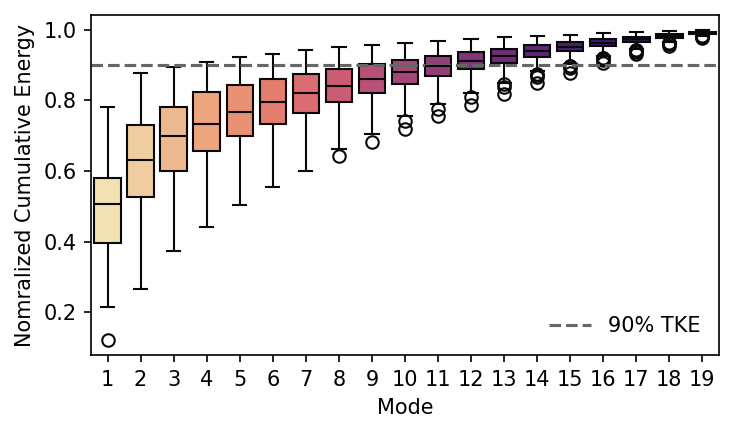
\includegraphics[width=0.6\textwidth]{figs/20240923.AWAKEN.cumLamNorm.png}
  \caption{The distribution of cumulative summations of eigenvalues associated with each case. Including }
  \label{fig:cumLamNorm}
\end{figure}

% TODO: add to discussion section too!
Because we apply the POD to each lidar data set independently, the resulting analysis produces a unique basis of modes for each case.
\Cref{fig:allModes} shows the POD modes associated with the case beginning at 2023-09-04 10:30 UTC.
Althought there are quantititive differences in the basis of modes for each case, qualitatively they are quite similar in structure and in order.
Colorbars are included with each mode, for completeness, although it should be noted that it is only when combined with the respecitive mode coefficients to form a ROM that the units and quantitative values are meaningful.

Because the POD is applied independently to each lidar dataset, the analysis generates a unique set of modes for each case. \Cref{fig:allModes} displays the POD modes for a specific case starting at 2023-09-04 10:30 UTC. 
While there are quantitative differences in the mode bases across cases, their structure and order remain qualitatively similar. Each mode is shown with a colorbar for completeness, although the units and quantitative values become meaningful only when combined with the corresponding mode coefficients to form a ROM.

\begin{figure}[h]
  \centering
  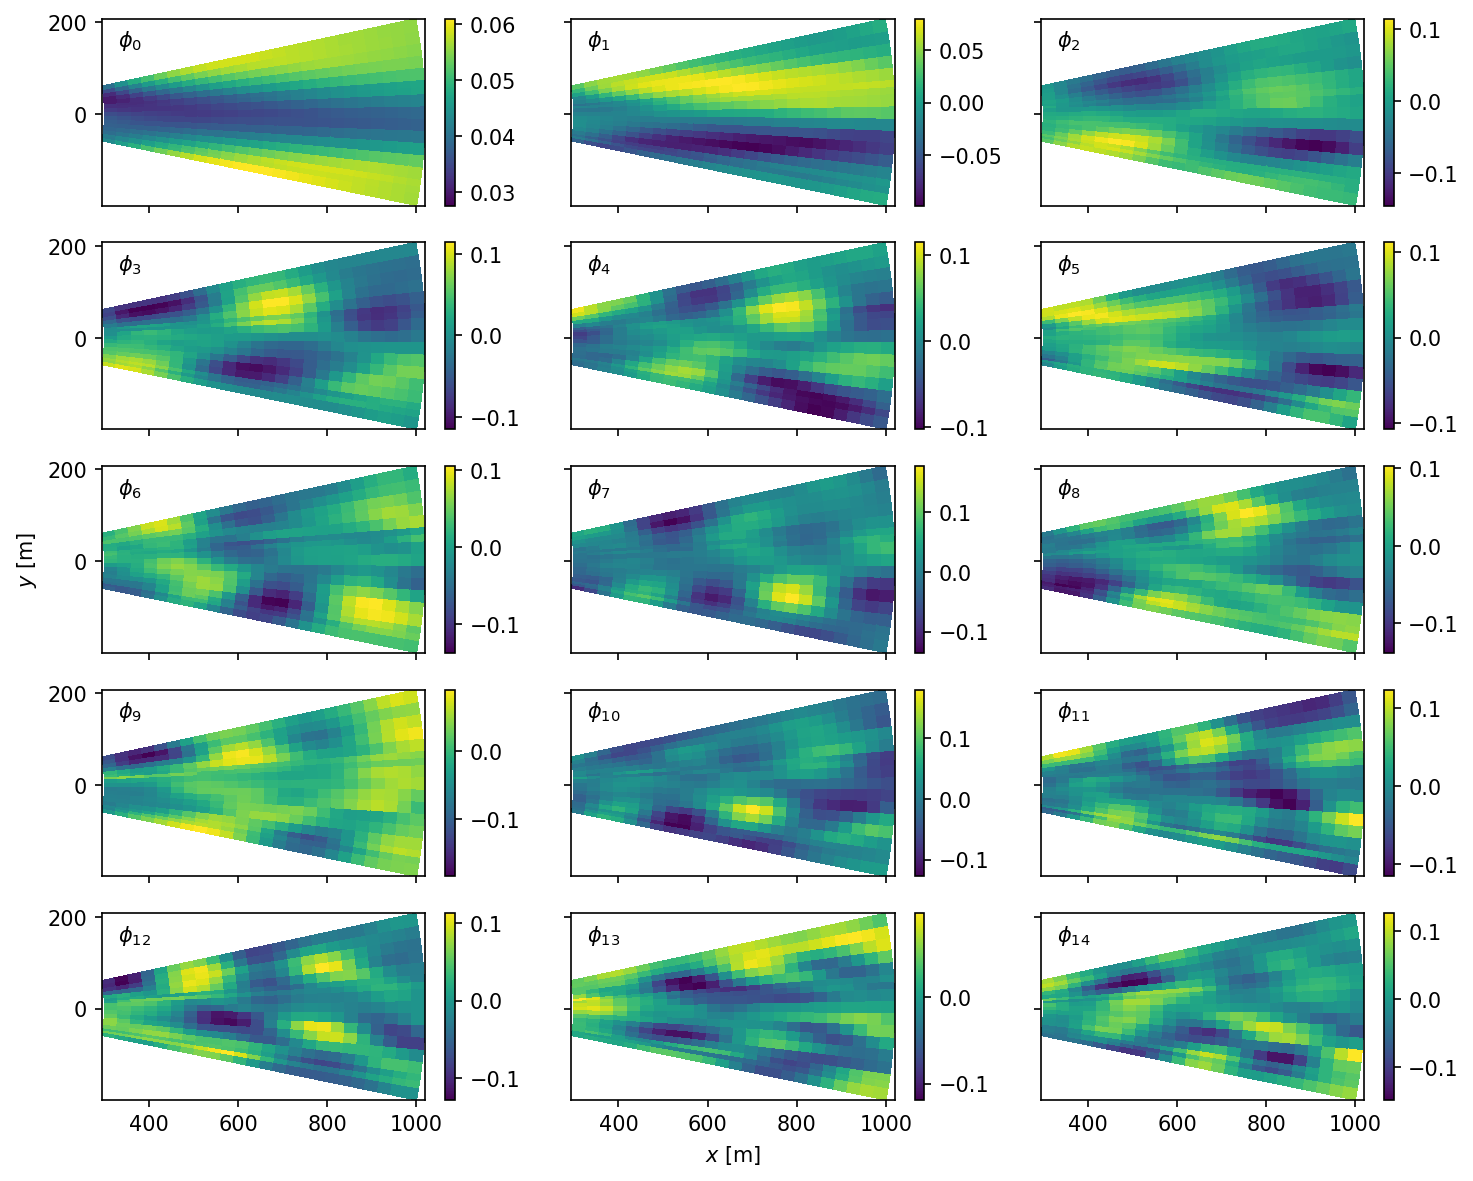
\includegraphics[width=\textwidth]{figs/20240826.AWAKEN.all.modes.png}
  \caption{POD modes from the example case on 2023-09-04 10:30 UTC.}
  \label{fig:allModes}
\end{figure}

The zeroth mode, $\phi_0$, represents the mean flow and clearly depicts the characteristic momentum deficit region of a wind turbine wake. 
Modes $\phi_1$ through $\phi_{14}$ describe coherent structures in the wake, ranked by their projection onto the lidar scans. 
The first mode, $\phi_1$, which accounts for approximately 20\% to 8\% of the TKE, captures large lateral shifts in the mean wake location and is most relevant for wake meandering. 
If we analogize the POD modes as Fourier modes, $\phi_2$, the second mode, describes a full oscillation in the streamwise ($x$) direction and a half oscillation in the transverse ($y$) direction. 
This mode, one order higher than $\phi_1$, represents the largest streamwise variations in the wake trajectory. 
Depending on the algebraic sign of its coefficient at any given time, $\phi_2$ may describe a shift toward positive $y$ near the turbine and toward negative $y$ farther downstream, or the reverse. 
The third mode, $\phi_3$, represents an additional half-period of oscillation, describing a period and a half in $x$ across the lidar scan domain.

From the fourth mode onward, it becomes increasingly difficult to relate the modes to specific changes in wake structure. 
For instance, $\phi_4$ is the first mode to display significant azimuthal asymmetry, complicating interpretation. 
In contrast, $\phi_5$ exhibits azimuthal symmetry, a first for the modes presented in \cref{fig:allModes}, but also displays a full oscillation along the $x$ direction, possibly reflecting vertical wake meandering projected onto the plane of the lidar scans. 
A mode describing two periods of vertical meandering is observed in $\phi_9$, further illustrating the complexity of higher-order modes.

% TODO: make a table descibing the mode structures, etc.
% \begin{table}[htbp]
%   \centering\begin{tabular}{cccc}
    
%   \end{tabular}
%   \caption{<caption>}
%   \label{<label>}
% \end{table}


%%%%%%%%% Bootstrapping modes for statistical convergence?
% Modes within thes bases for each case do not converge at the same rate. 
% Lower-rank modes describe turbulent structures represented in more observations, by definition, and converge faster. 
% Higher ranking modes represent less coherent structures, accounting for less variance within the basis of lidar scans, and require a larger sample size to be statistically converged. 
% \Cref{fig:convergence} contains the results of a convergence test that compares the variability of POD modes constructed from randomly sampled snapshots within the set of observations, averaging over all three test cases. 
% The mode error, $\varepsilon_{\phi^{(i)}}$, shown in \cref{fig:convergence} is defined as the standard deviation of POD modes defined with a randomly selected sample of $N$ snapshots. For each basis size $N$, up to 1000 subsets of observations were used to define POD bases, offering a statistical view of the structures described by the POD modes. 


In reconstructing the flow field following \cref{eq:PODset}, between 3 and 14 POD modes were used to describe the turbulence, in addition to the mean flow described in $\phi_0$. 
For each case, all 16,278 possible mode combinations were tested, producing a large sample of reconstructed wakes, each described by a unique subset of the modes from $\phi_1$ to $\phi_{14}$. 
\Cref{fig:modesPerRom} illustrates the mode combinations used in each ROM, with ROMs defined by only four modes (the mean flow $\phi_0$ and three turbulent modes between $\phi_1$ and $\phi_{14}$) displayed on the left, and those incorporating more modes shown on the right. 
For each combination, the wake profiles were fitted to the Gaussian function in \cref{eq:gaussfit}, and a low-order estimate of the lateral wake center, $\hat{\mu}$, was extracted.

\begin{figure}[h]
  \centering
  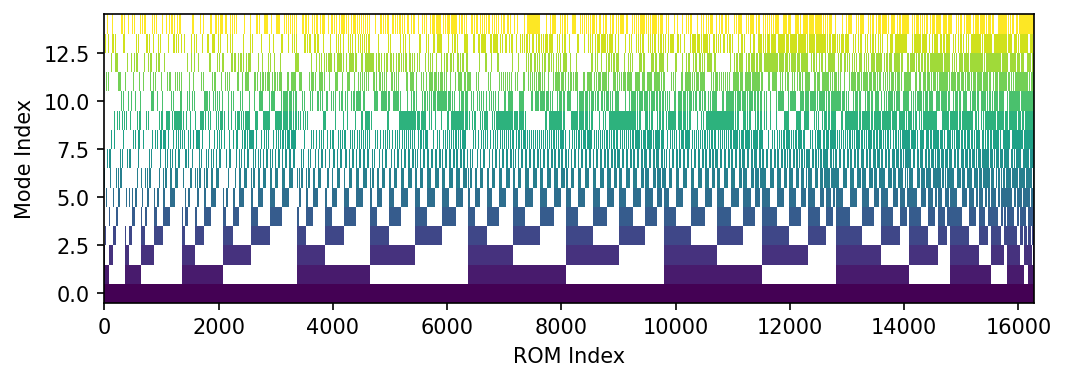
\includegraphics[width=\textwidth]{figs/modesPerRom_20240828.png}
  \caption{Combination tree indicating which modes are contained in any given ROM. Modes are indicated by the colored regions, and their absence is shown in white. \comment{change cbar label}}
  \label{fig:modesPerRom}
\end{figure}

When reconstructing the velocity field using POD modes, our objective is to match the power spectral density (PSD) of wake center locations from the reconstructed flow field, $S_{\hat{\mu}\hat{\mu}}$, as closely as possible to that of the original field, $S_{\mu\mu}$. 
Mode combinations that accurately reproduce wake meandering for each case (i.e., where $S_{\mu\mu} \approx S_{\hat{\mu}\hat{\mu}}$) are considered representative of wake meandering in the low-order velocity field representation. 
Coherence, defined in \cref{eq:coh}, quantifies the similarity between wake center trajectories in the lidar scans and the ROMs. 
\begin{equation} 
  C_{\mu \hat{\mu}}(f, x) = \frac{|S{\mu\hat{\mu}r}(f, x)|^2}{S{\mu\mu}(f, x) S{\hat{\mu}\hat{\mu}}(f, x)} 
  \label{eq:coh} 
\end{equation} 
In this context, coherence $C_{\mu \hat{\mu}}(f, x)$ measures the similarity of the wake center dynamics at frequency $f$, where $C_{\mu \hat{\mu}}(f, x) = 1$ indicates a perfect match between the PSDs of the wake centers, and $C_{\mu \hat{\mu}}(f, x) = 0$ indicates no match.

% In practice, $C_{\mu \hat{\mu}}(f, x)$ depends on both the frequency and the downstream distance under consideration. 

As a general trend, the PSDs of the wake centers show better agreement at lower frequencies ($f_s < St_{in}$ Hz), which are more accurately captured by the POD modes used in the ROMs. 
Coherence decreases at higher frequencies, but because wake meandering is predominantly a low-frequency phenomenon, this reduction in coherence at higher $f_s$ is acceptable for the purposes of this study.
To illustrate this, \cref{fig:bestWorstSpectra} shows the average coherence over the full frequency range for several cases, which demonstrate good agreement between $S_{\mu\mu}$ and $S_{\hat{\mu}\hat{\mu}}$, particularly for $x/D > 4$. 
The highlighted regions in \cref{fig:bestWorstSpectra} indicate the region where $f_s < St_{in}$, that is where the reduced frequency is less than twice the inflow Strouhal number.
Considering only part of the total frequency range of $C_{\mu \hat{\mu}}$ gives a more accurate representation of the quality of any particular ROM to reproduce wake meandering in particular---the high frequency rnage of the spectra is not relevant to wake meandering as the physics of interest.
The trends for both ROMs in \cref{fig:bestWorstSpectra} were evaluated by calucalting the average coherence, $\overline{C_{\mu \hat{\mu}}}$, over the respective frequency range.

\begin{figure}[htbp]
  \centering
  \begin{subfigure}[b]{0.49\columnwidth}
    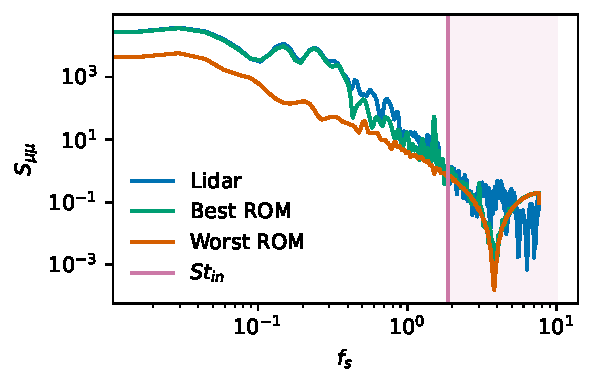
\includegraphics[width=\columnwidth]{figs/20241203.romSpectra.pdf}
  \end{subfigure}
  \begin{subfigure}[b]{0.49\columnwidth}
    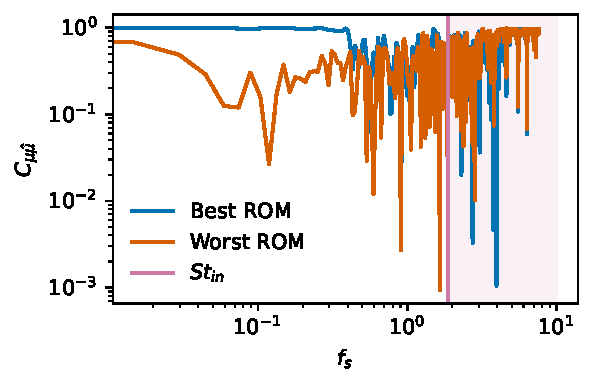
\includegraphics[width=\columnwidth]{figs/20241203.romCoherenceSpectra.pdf}
  \end{subfigure}
  \caption{Spectra (left) and coherence (right) for the ROMs that compare best (green) and worst (orange) to the PSD of $\mu$ from the lidar scans. }
  \label{fig:bestWorstSpectra}
\end{figure}


A more complete picture of ROM quality is provided in \cref{fig:meanCoherence}, which shows the coherence averaged over the reduced frequency, $\overline{C}_{\mu \hat{\mu}}$.
The top subfigure shows $\overline{C}_{\mu \hat{\mu}}$ considering the full frequency range, and suggests that the average coherence is around 0.3 for most cases.
In contrast, the bottom subfigure shows $\overline{C}_{\mu \hat{\mu}}$ considering only $f_s \le St_{in}$, and shows much more consistent results for blocks of ROMs.
Recalling the distribution of modes considered in each ROM presented in the combination tree shown in \cref{fig:modesPerRom}, a correlation between $\overline{C}_{\mu \hat{\mu}}$ and the presence of certain modes becomes clear.

\begin{figure}[htbp]
  \centering
  \begin{subfigure}[b]{0.9\columnwidth}
    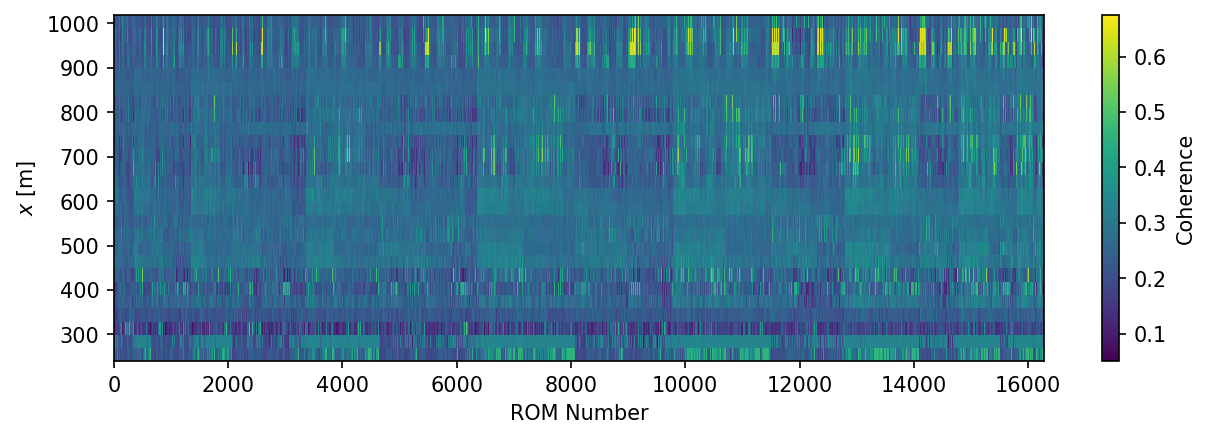
\includegraphics[width=\columnwidth]{figs/20240927.AWAKEN.averageCoherence.png}
  \end{subfigure}
  \begin{subfigure}[b]{0.9\columnwidth}
    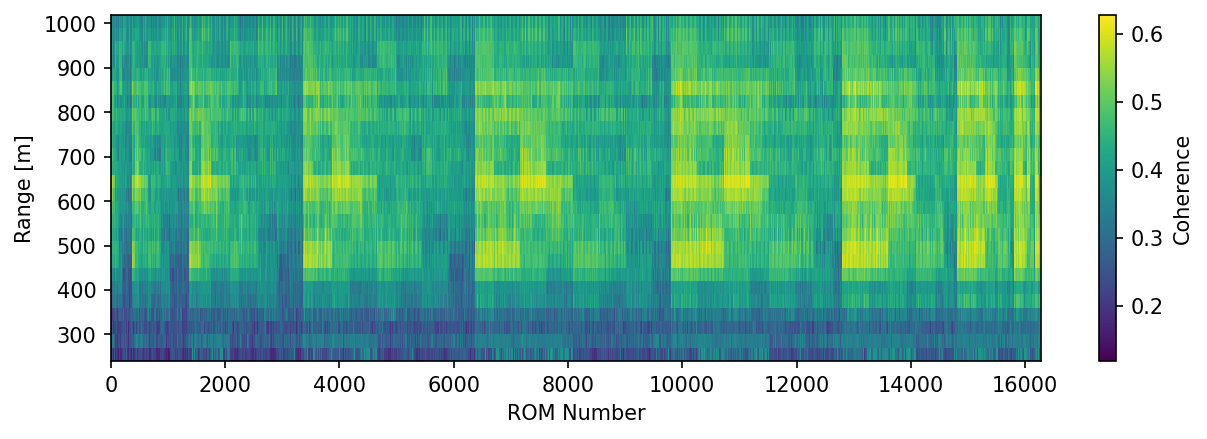
\includegraphics[width=\columnwidth]{figs/20240925.AWAKEN.meanMeanderingCoherence.png}
  \end{subfigure}
  \caption{Frequency-average coherence between detected wake centers from lidar scans and ROMs considering the full measured frequency range (top) and only frequencies $f_s \le St_{in}$ Hz (bottom).}
  \label{fig:meanCoherence}
\end{figure}

The information contained in \cref{fig:meanCoherence} also indicates dependence of $\overline{C}_{\mu \hat{\mu}}$ on the downstream distance away from the lidar, as shown in the vertical axes.
Aggregating this information into a single scalar metric for each ROM by averaging along the range coordinate, $\varepsilon = \langle \overline{C}_{\mu \hat{\mu}} \rangle$, we are able to describe the distribution of ROMs in terms of a quantitative metric for fit quality.
\Cref{fig:RangeMeanCoherence} (left) shows $\varepsilon$ arranged by the index of the ROM, spanning the 16,278 mode combinations.
The data in \cref{fig:RangeMeanCoherence} represent the the same data shown in \cref{fig:meanCoherence}, averaged over the streamwise coordinate (vertical plot axis).
Aggregated a different way, \cref{fig:RangeMeanCoherence} (right) shows the distribution of the ROM quality according to the number of modes used in the definition of each ROM.
While the overall trend suggests that inclduing more modes in a ROM generally increases the quality of the representation of wake meandering, it is interesting to note that there are plenty of exceptions to this trend.
The distributions in \cref{fig:RangeMeanCoherence} (right) indicate several ROMs with only four modes outperfom some of the ROMs with 14 modes.

\begin{figure}[htbp]
  \centering
  \begin{subfigure}[b]{0.49\columnwidth}
    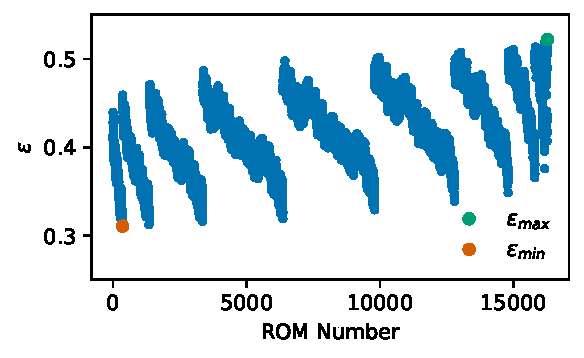
\includegraphics[width=\columnwidth]{figs/20241204.vareps_by_ROM.pdf}
  \end{subfigure}
  \begin{subfigure}[b]{0.49\columnwidth}
    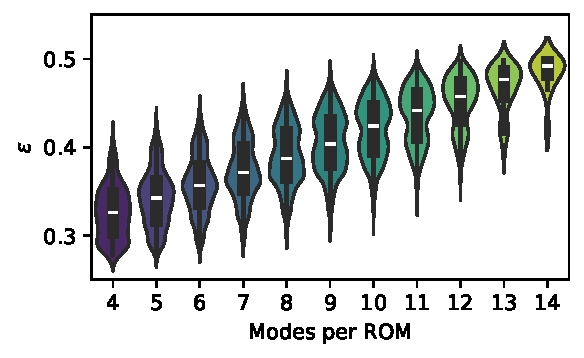
\includegraphics[width=\columnwidth]{figs/meanderCoherenceByNModes_20240927.pdf}
  \end{subfigure}
  \caption{Frequency and range-averaged coherence between detected wake centers from lidar scans and ROMs considering $f_s \le St_{in}$ Hz (left). Distribution of $\varepsilon$ by the number of modes contained in each ROM (right). \comment{make vertical scales identical}}
  \label{fig:RangeMeanCoherence}
\end{figure}


To evaluate the influence of individual POD modes on wake meandering, we perform a linear regression analysis using the full set of 16,287 mode combinations for each case. 
Given that each low-dimensional flow field representation is a linear combination of POD modes and their corresponding coefficients, the reconstructed flow field $\hat{u}$ is inherently linearly dependent on the included modes. 
The sensitivity of the wake center location to the inclusion or exclusion of specific modes was examined through a linear regression of modes (as dummy variables) against the average coherence between $\mu$ and $\hat{\mu}$, $C_{\mu \hat{\mu}}(f, x)$.

% The linear system can be expressed as:
% \begin{equation}
%   \bm{\varepsilon} = \bm{X}\bm{\beta} + \xi
%   \label{eq:linearreg}
% \end{equation}
% where the vector $\bm{\varepsilon} = [\varepsilon_1, ..., \varepsilon_K]$ contains the streawise and frequency averaged coherence for each ROM mode combination, $\bm{X} = [I_1, ..., I_K]$ is the matrix of mode combinations for up to $K=16,278$ combinations in each case, and $\bm{\beta} = [\beta_1, ..., \beta_K]$ contains the regression coefficients for each mode. 
% The term $\xi$ represents the residual error of the regression.

% The regression coefficients for modes 1 through 14 are shown in \cref{fig:modeSensitivity}.
% Following the intuitive understanding of the physics underlying the modes, the coefficient $\beta_1$, describing the linear sensitvity of $\varepsilon$ to $\phi_1$ is much larger than coefficients for other modes.

% \begin{figure}[htbp]
%   \centering
%   \begin{subfigure}[b]{0.48\columnwidth}
%     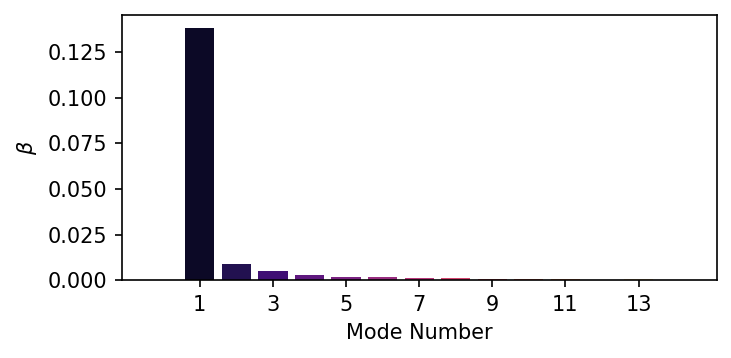
\includegraphics[width=\columnwidth]{figs/20230904.AWAKEN.modeRelevance.case1030.20240930.png}
%   \end{subfigure}
%   \begin{subfigure}[b]{0.48\columnwidth}
%     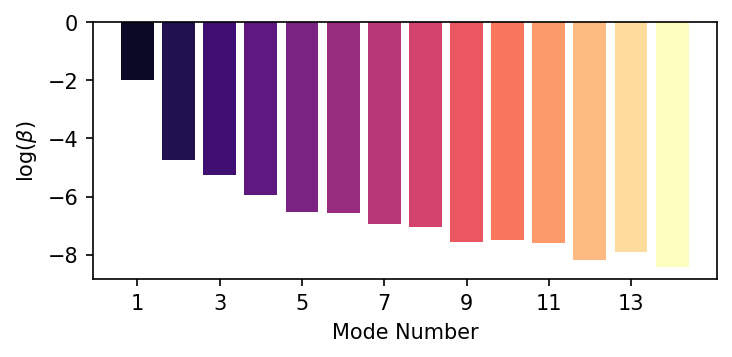
\includegraphics[width=\columnwidth]{figs/20230904.AWAKEN.log.modeRelevance.case1030.20240930.png}
%   \end{subfigure}
%   \caption{Sensitivity of ROM accuracy to paricular modes for the 2023-09-04 10:30 UTC case. Sensitivity coefficients are shown in linear (left) and logarithmic (right) scales.}
%   \label{fig:}
% \end{figure}

% As depicted in \cref{fig:modeSensitivity}, certain nonsequential structures consistently influence the standard deviation of the detected wake center.
% Large positive values of $\beta$ indicate modes that most significantly contribute to accurately reproducing wake meandering in $\hat{u}$ as described by $\varepsilon$. 
% Conversely, negative values of $\beta$ indicate modes that somehow increase the error in reconstructed wake meandering.

% \begin{figure}[h]
%   \centering
%   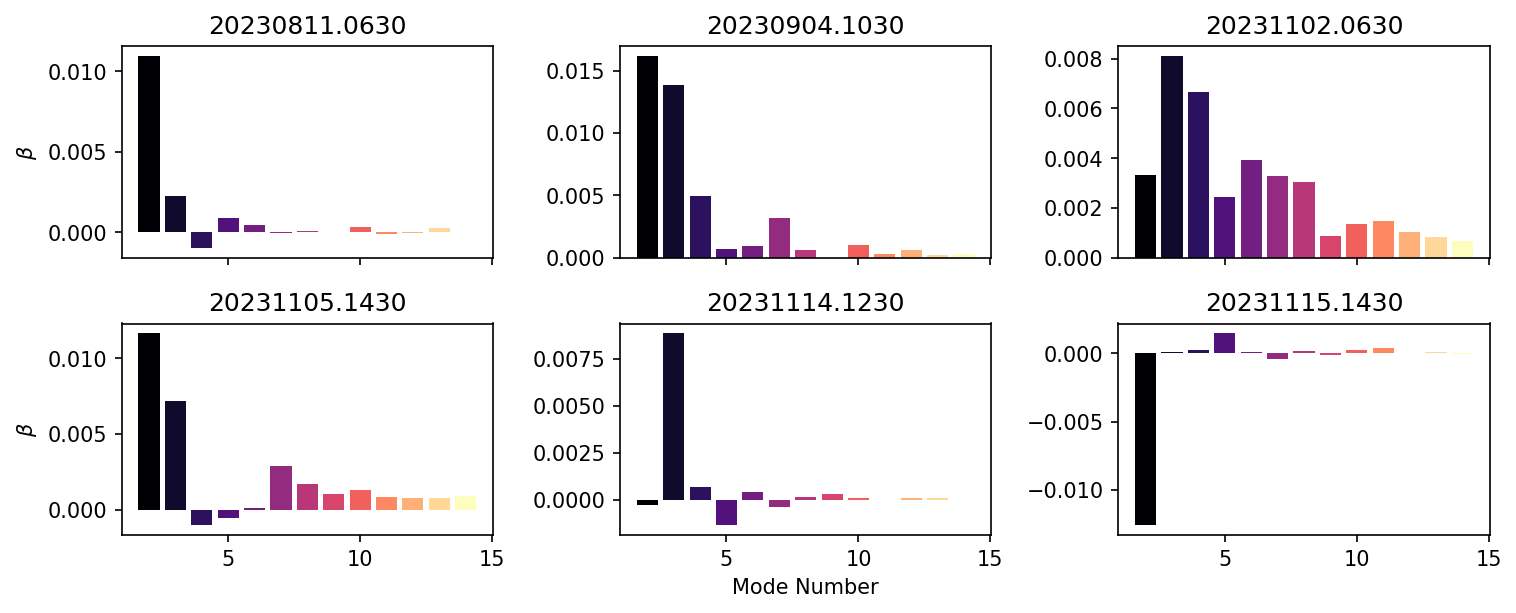
\includegraphics[width=\textwidth]{figs/20240930.AWAKEN.mode.sensitivity.cases.png}
%   \caption{Sensitivity of the coherence in the meandering frequecy ranges to presence/absense of POD modes for selected cases.}
%   \label{fig:modeSensitivity}
% \end{figure}

The sensitivity of the wake center coherence to POD modes was investigated using an Analysis of Variance (ANOVA\cite{sahaiAnalysisVarianceFixed2012}) approach. 
We develop a statistical model to decompose the observed coherence metric into contributions from individual modes and their interactions.
The model takes the form of a linear decomposition, where the average coherence $\varepsilon$ as a quality metric for each ROM is expressed as a function of mode presence, accounting for both individual mode effects and two-way interactions:
\begin{equation}
\varepsilon = \overline{\varepsilon} + \sum_{i=1}^{n} \beta_i q_i + \sum_{i<j}^{n} \gamma_{ij} q_i q_j + \xi
\label{eq:anova}
\end{equation}
where, $\overline{\varepsilon}$ represents the global mean coherence for each case, $\beta_i$ are the main effects of individual modes, and $\gamma_{ij}$ capture the interaction effects between modes. 
The binary variables $q_i$ indicate the presence (1) or absence (0) of each mode, with a constraint that at least three modes must be included. The term $\epsilon$ represents the residual error.

We impose statistical constraints assuming that both the main effects $\beta_i$ and interaction terms $\gamma_{ij}$ follow a normal distribution with zero mean, and that the residual error $\epsilon$ follows a normal distribution. 
The objective is to estimate the coefficients $\beta_i$ and $\gamma_{ij}$ that minimize the residual error while providing insight into how different modes and their combinations influence the wake center coherence.
This approach allows for a comprehensive sensitivity analysis that goes beyond simple linear contributions, capturing the complex, potentially non-linear interactions between POD modes in representing the wake center dynamics.

\begin{figure}[htbp]
  \centering
  \begin{subfigure}[b]{0.6\columnwidth}
    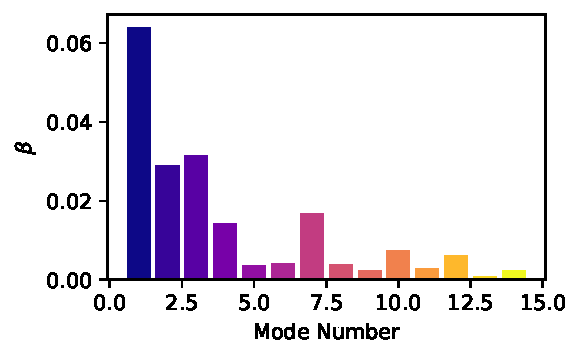
\includegraphics[scale=0.9]{figs/20241203.modeEffectBar.pdf}
  \end{subfigure}
  \begin{subfigure}[b]{0.39\columnwidth}
    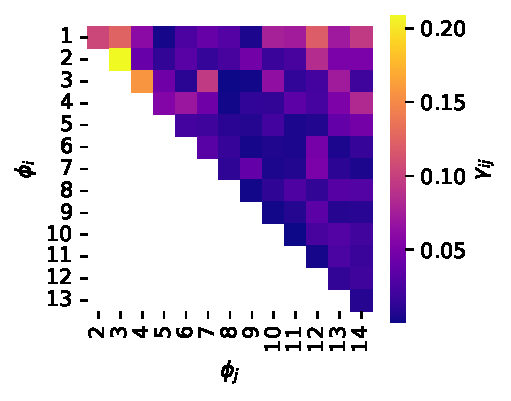
\includegraphics[scale=0.84]{figs/20241203.modeInteractionHeatMap.pdf}
  \end{subfigure}
  \caption{}
  \label{fig:anovaCaseStudy}
\end{figure}

\begin{figure}[h]
  \centering
  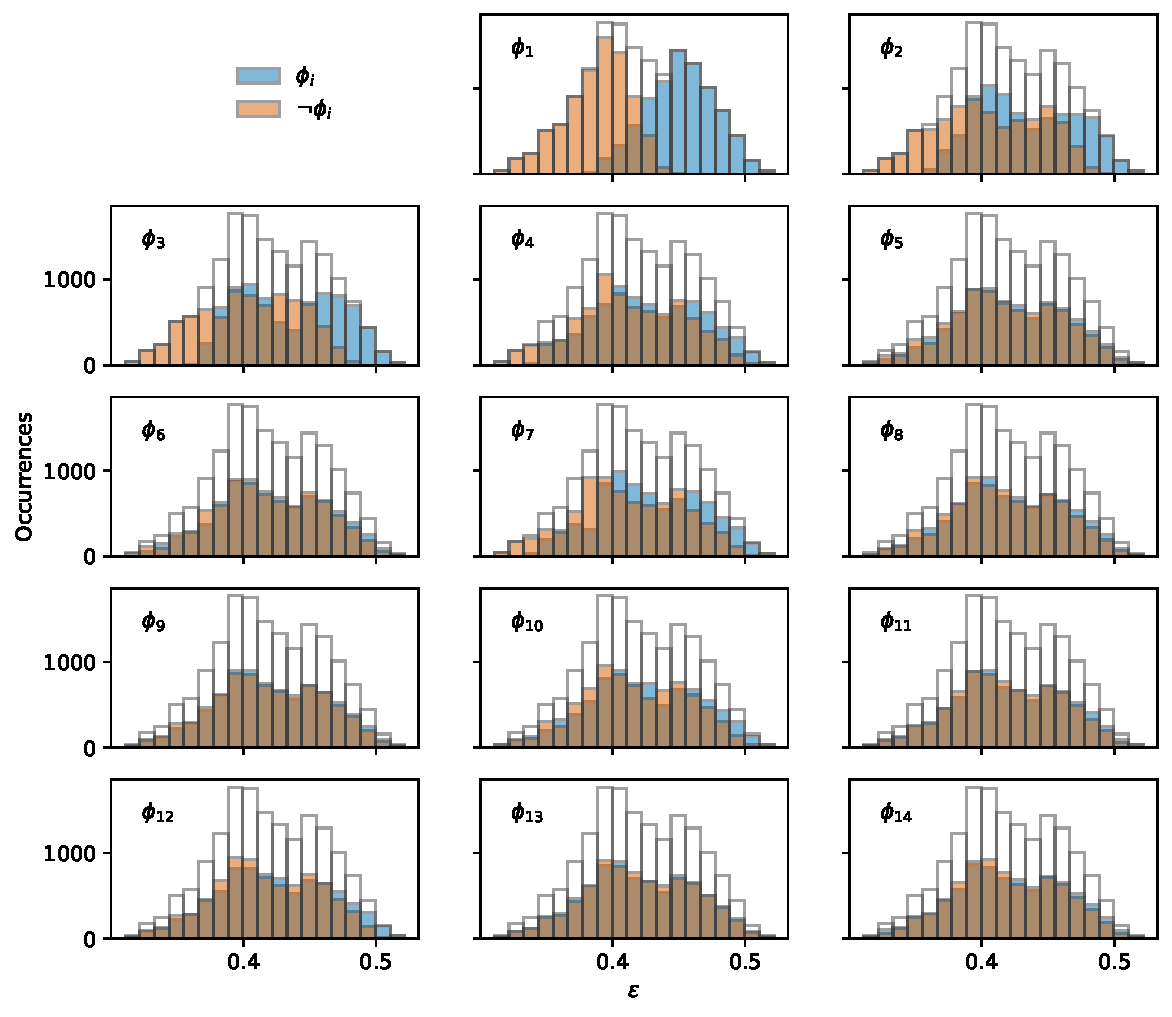
\includegraphics[width=\textwidth]{figs/20241203.vareps.allmodes.pdf}
  \caption{}
  \label{fig:vareps_by_modeBeta}
\end{figure}

\begin{figure}[h]
  \centering
  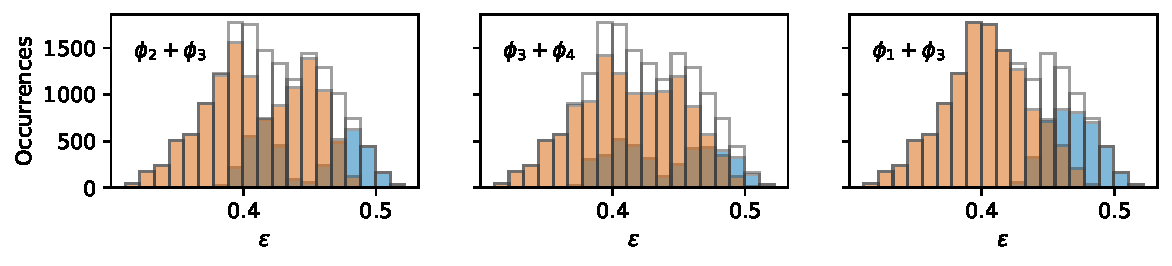
\includegraphics[width=\textwidth]{figs/20241203.vareps.highGammaPairs.pdf}
  \caption{}
  \label{fig:highGammaPairs}
\end{figure}

\begin{figure}[htbp]
  \centering
  \begin{subfigure}[b]{0.45\columnwidth}
    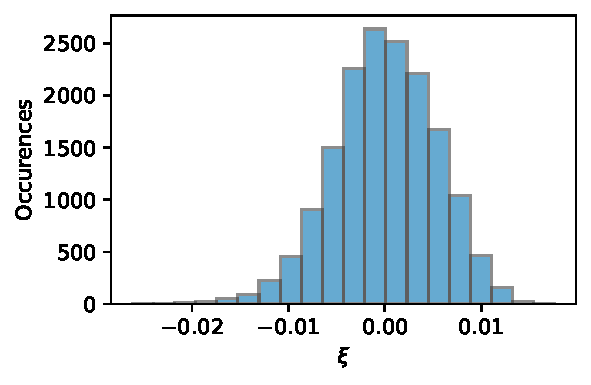
\includegraphics[width=\columnwidth]{figs/20241205.residualHist.pdf}
  \end{subfigure}
  \begin{subfigure}[b]{0.48\columnwidth}
    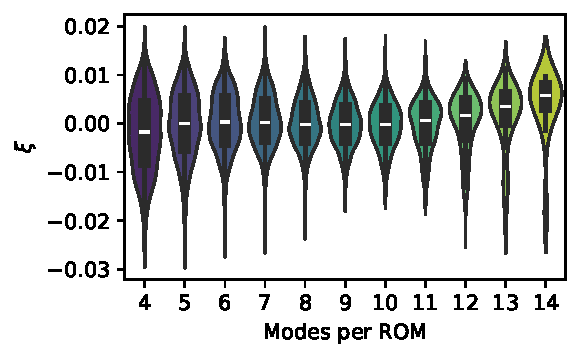
\includegraphics[width=\columnwidth]{figs/20241205.residual_byNmodes.pdf}
  \end{subfigure}
  \caption{}
  \label{fig:}
\end{figure}

\begin{figure}[htbp]
  \centering
  \begin{subfigure}[b]{0.48\columnwidth}
    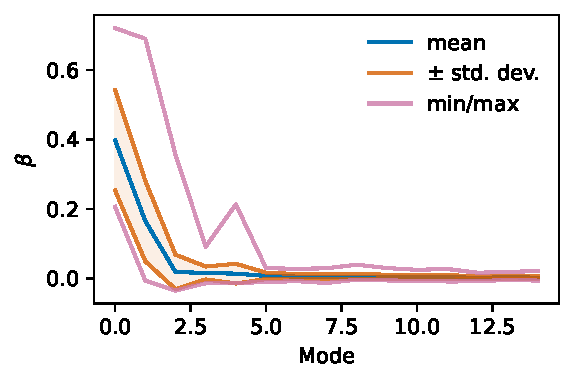
\includegraphics[width=\columnwidth]{figs/20241204.beta.meanRange.pdf}
  \end{subfigure}
  \begin{subfigure}[b]{0.48\columnwidth}
    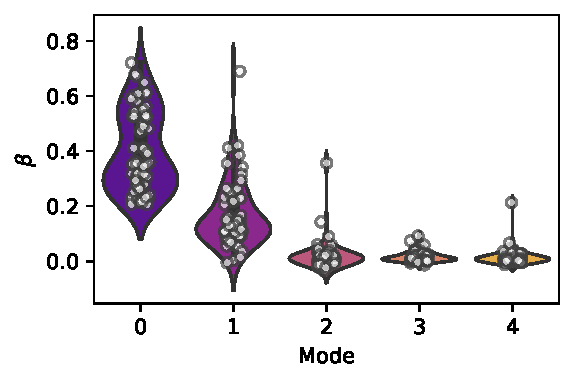
\includegraphics[width=\columnwidth]{figs/20241204.beta.violinJitter.pdf}
  \end{subfigure}
  \caption{}
  \label{fig:}
\end{figure}

\begin{figure}[htbp]
  \centering
  \begin{subfigure}[b]{0.48\columnwidth}
    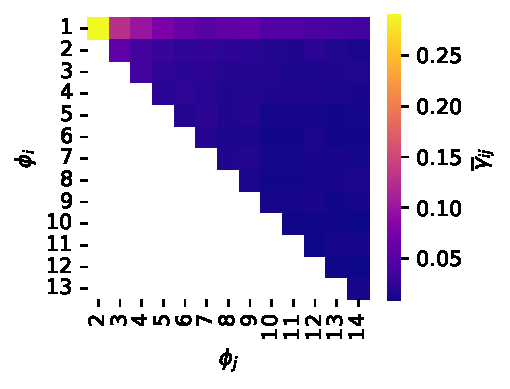
\includegraphics[width=\columnwidth]{figs/20241203.modeInteractionHeatMap_mean.pdf}
  \end{subfigure}
  \begin{subfigure}[b]{0.48\columnwidth}
    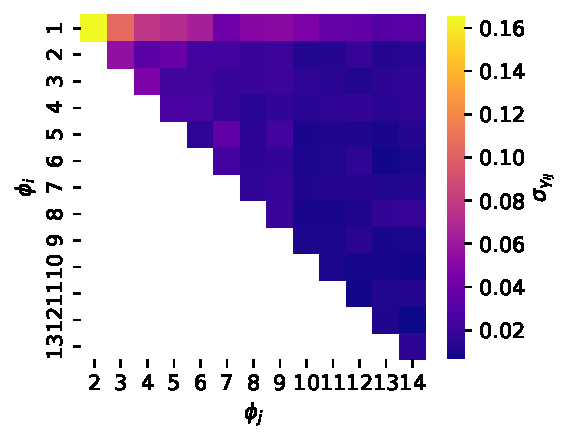
\includegraphics[width=\columnwidth]{figs/20241203.modeInteractionHeatMap_std.pdf}
  \end{subfigure}
  \caption{}
  \label{fig:}
\end{figure}

\begin{figure}[h]
  \centering
  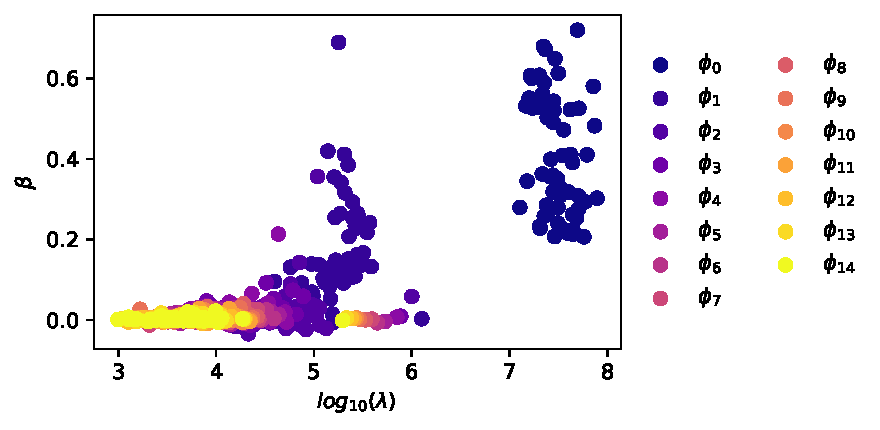
\includegraphics[width=0.7\textwidth]{figs/20241204.lamda_v_beta.pdf}
  \caption{}
  \label{fig:}
\end{figure}

% \Cref{fig:bestworst} illustrates selected turbulence structures underlying the regression test results for Case C in \cref{fig:regression}. 
% In the left column, modes 1, 2, and 5 are those that contribute most to the accurate reconstruction of wake meander. 
% Each of the structures for modes 1, 2, and 5 occupy the full scan area and exhibit some asymmetry over the streamwise axis that contributes to the variability in the wake center location.
% In the right column, the structures have a more complicated spatial character, highlighting many smaller regions within the scan area. 
% When integrated into a reconstructed flow field as in \cref{eqn:nuts}, these structures do not contribute significantly to the meandering of the wake center. 

% \begin{figure}[h]
%   \centering
%   \begin{subfigure}[b]{0.45\columnwidth}
%     \includegraphics[width=\columnwidth]{figs/C_best_modes.png}
%     % \caption{Normalized POD eigenvalues}
%     % \label{fig:eig}
%   \end{subfigure}
%   \hspace{0.5cm}
%   \begin{subfigure}[b]{0.45\columnwidth}
%     \includegraphics[width=\columnwidth]{figs/C_worst_modes_20210818.png}
%     % \caption{Cumulative summation of eigenvalues}
%     % \label{fig:cumsum}
%   \end{subfigure}
%   \caption{Modes contributing the most (left) and the least (right) to the accurate reproduction of wake meander.}
%   \label{fig:bestworst}
% \end{figure}



% For visual verification of the regression findings presented above, \cref{fig:fieldrec} compares the velocity field from Case C presented by the lidar scan (left) to the best (center) and worst (right) reconstructions with 6 modes and the time averaged flow field.
% This particular case and value of $k$ (Case C and $k=7$) was selected to highlight the differences between the best and worst combinations of modes, with the maximum difference between streamwise averaged $\Delta \sigma_c$.
% In \cref{fig:fieldrec}, the contour plot denotes the velocity field, with the wake highlighted with brighter colors and freestream velocity in black.
% Superimposed on the flow field, the detected wake center for this particular scan are shown with white markers.
% Detected wake centers for the best reconstruction (center) closely match those of the original lidar scan, with the exception of $x/D=3$, very close to the turbine.
% This in itself is interesting as the near wake was shown in \cref{fig:centerdist} to exhibit the least variability. 
% That the best-fit reconstruction misses the near wake may indicate that particular modes are better suited to represent the wake center distribution near the turbine, and others better for the far wake.
% The worst-fit reconstruction (right) does not accurately represent either the flow field or the wake centers. 

% \begin{figure}[h]
%   \centering
%   \includegraphics[width=\textwidth]{figs/C_rec_best_worst.png}
%   \caption{Velocity field from Case A (left) along with the best (center) and worst (right) reconstructions with 7 modes.}
%   \label{fig:fieldrec}
% \end{figure}

% The inflow Strouhal number, $St_\text{in}=D/U_\text{hub}\cdot T $, defined with the rotor diameter, the hub-height inflow velocity, and the inverse of the integral time scale represents the cutoff frequency for the externally-driven meandering hypothesis.
% In this hypothesis, any turbulent motions in the inflow occurring at a frequency at or below $St_\text{in}$ are assumed to carry the momentum deficit of the wake as a passive tracer.
% In practice, this requires that any the frequencies of the wake meandering must also be at or below the inflow Strouhal number. 
% The comparison of $St_\text{in}$ to spectra of the detected wake centers  ($S_\text{wake}$) in \cref{fig:wakeSpectra} does not show an entirely clear picture of the response for $x/D \in [3,6,9]$.
% While the peaks of spectra, shown as dots, for Cases B and C (orange and gray) occur below $St_\text{in}$, shown as vertical lines, this relationship does not hold for Case A.
% The cause for the unexpected behavior in the wake center location spectra for Case A is not immediately clear, but may be related to the change of operating conditions seen during that time period. 

% \begin{figure}[htb]
%     \centering
%     \includegraphics[width=\columnwidth]{figs/wake_spectra.png}
%     \caption{Wake center spectra from the lidar scans in Strouhal scaling. The vertical line in each plot shows $St_\text{in}$ for Cases A, B, and C, from left.}
%     \label{fig:wakeSpectra}
% \end{figure}

% POD modes themselves are functions only of space, all time dependence of each structure is contained in the mode amplitudes $a_i(t)$, as in \cref{eqn:POD}.
% Computing the power spectral density (PSD) for each mode coefficient ($S_{a_i}$) highlights the spectral contribution of each mode in the reduced-order description of the wake.
% For each mode, the Strouhal number associated with the maximum value of the PSD is taken as the characteristic dimensionless frequency for each mode, $St_\text{wake}$, noting that the maximum frequency resolved is half that of the the lidar scans $f_\text{max} = f_\text{scan}/2 \approx  0.07$ Hz. For each mode coefficient, frequencies are described in Strouhal scaling as $St = f\cdot D/U_\text{hub}$.

% The maximum Strouhal number for each mode depends on the average hub-height velocity for each case. 
% \Cref{fig:bestworstcoeff} shows the PSDs of the POD coefficients associated with the modes highlighted by the regression coefficients in \cref{fig:regression}.
% For each case, the modes most closely associated with wake meandering---those with the largest negative values of $\beta$---are shown on the left. 
% PSDs of coefficients that contribute least to the reconstruction of wake meandering are shown on the right.
% Note that modes are listed in the order of the greatest (left) and least (right) contributions, and are different for each case.
% For each mode, a point of the same color indicates the maximum value of the PSD and the characteristic Strouhal number, $St_{a_i, \text{c}}$.

% \begin{figure}[h]
%   \centering
%   \begin{subfigure}[b]{0.49\columnwidth}
%     \includegraphics[width=\columnwidth]{figs/best_coeff_mt.png}
%   \end{subfigure}
%   \begin{subfigure}[b]{0.49\columnwidth}
%     \includegraphics[width=\columnwidth]{figs/worst_coeff_mt.png}
%   \end{subfigure}
%   \caption{PSDs of POD projection coefficients ($a_i$) for the modes that contribute most (left) and least (right) to wake meandering.}
%   \label{fig:bestworstcoeff}
% \end{figure}

% The spectra shown in \cref{fig:bestworstcoeff} associated with an accurate representation of wake meandering (left) consistently show peaks of $St_{a_i, \text{c}} < 0.2$, agreeing with dominant meandering frequencies in previous work,
% \cite{medici2008measurements,okulov2007stability, okulov2014regular,howard2015statistics,foti2016wake,foti2018wake,baker1985wake,zambrano1983wake,larsen2007dynamic,larsen2008wake,jonkman2017development}
% but the relationship is less clear for modes that contribute little to meandering (right).
% \Cref{fig:ST_comp} compares the $St$ associated with spectral peaks for the POD modes in all cases to those of the inflow (solid lines) and those observed in the wakes (dashed lines).
% Spectral peaks shown with open diamonds are those from the POD modes that correspond most with the accurate reconstruction of the wake meandering, filled circle markers are all other modes considered for velocity field reconstruction.
% \begin{figure}[htb]
%     \centering
%     \includegraphics[width=0.8\columnwidth]{figs/ST_comparison.png}
%     \caption{Peak $St$ derived from POD mode coefficients for each case. Diamond markers are the modes that contribute most to meander, circle markers are modes that contribute less. The solid vertical lines are $St_\text{in}$, dashed vertical lines are $St_\text{wake}$.}
%     \label{fig:ST_comp}
% \end{figure}
% As with the spectra in \cref{fig:wakeSpectra}, the results comparing $St_{a_i,\text{c}}$ for individual modes in \cref{fig:ST_comp} are not entirely consistent with the externally-driven meandering hypothesis. 
% For that to be the case, we would expect $St_{a_i,\text{c}}$ to be more cleanly divided by $St_\text{in}$, with modes that contribute to the accurate reconstruction of the wake (diamonds) at $St_{a_i,\text{c}} < St_\text{in}$ and modes that contribute little to meandering to have $St_{a_i,\text{c}} > St_\text{in}$.
% Instead, we see a mix of $St_{a_i,\text{c}}$, where some of the modes that contribute least to meander have the lowest characteristic frequencies.

% Similarly, following the internally-driven meandering hypotheses, those that assert that wake meandering is a product of interactions between turbulent structures in the wake, we would expect modes that contribute to meandering to have frequencies near those of the wake meandering detected from the lidar scans.
% Because the POD identifies coherent turbulent structures, like hub and tip vortices, it is reasonable to expect that their interactions should be characterized by the POD modes and coefficients. 
% However, values of $St_{a_i,\text{c}}$ do not show any consistent behavior related to $St_\text{wake}$ either.
% Although tip and hub vortices are typically associated with characteristic frequencies higher than are resolved with the lidar scans, their interactions should be on the same order of magnitude as the wake meandering. 



\section{Conclusions} % (fold)
\label{sec:Conclusions}


% The use of remote sensing data  from scanning lidars in wind turbine wake research gives us an opportunity to examine wake dynamics at full scale. 
% Measurements are guaranteed to align with the atmospheric flow and with the wind turbine wake by mounting the lidar on the nacelle.
% This work uses high-speed horizontal sector scans from a nacelle-mounted lidar to assess the wake meandering dynamics of a utility scale wind turbine operating in three different inflow conditions.
% Wake center locations, detected downstream of the wind turbine by fitting a Gaussian profile to the wake, show different meandering statistics in each of the test cases.
% In this work, we quantify wake meandering in a spatiotemporal sense with snapshot POD and in a spectral sense by seeking characteristic dimensionless meandering frequencies. 

% The Snapshot POD describes coherent turbulent structures in the wake, along with their relative contribution to the overall TKE budget and a coefficient that describes their dynamics.
% In this work, we exhaustively examine the reconstructed wake flow by selecting subsets of POD modes in a combinatorial sense, and compare meandering statistics to those shown in the lidar scans.
% Our work shows that, contrary to expectation, the lowest ranking modes do not necessarily contribute most to the accurate representation of wake meandering.
% Although the lowest order modes represent the largest, most coherent turbulent structures, they are not uniformly present in the combinations that best represent wake meandering. 

% Low-dimensional representations of the flow field are simply linear combinations of POD modes and their respective coefficients, indicating that the final flow field depends linearly on each mode.
% A regression test between modes and meandering statistics suggests that some modes are completely disconnected from meandering dynamics, and still others that actively work \emph{against} accurately representing wake meandering in low-dimensional flow reconstructions.
% Moreover, some of the best-fit reconstructions may consistently fail to accurately describe the wake center at particular downstream locations depending on the modes used in the low-order description, indicating that some modes are relevant to different regions of the wake.

% However, spectra defined from the mode coefficients most correlated with describing wake meandering do not exhibit the expected relationship with the characteristic Strouhal numbers of the inflow or of the wake.
% Dynamics wake meandering models that treat the momentum deficit in the wake as a passive tracer assume that wake motion is driven by atmospheric turbulence above a certain cutoff frequency, and so the Strouhal numbers for significant modes should be lower than that of the inflow.
% Those that say wake meandering is a product of the interaction between coherent turbulent structures in the wake should expect to see a relationship between the characteristic Stouhal numbers of the wakes and those of the modes.
% Unfortunately, neither relationship is evident in the results of the current study, either because the structures that describe meandering are not adequately resolved by the measurements, or because wake meandering has a more complex relationship with turbulence in the wake and inflow than noted in the literature.

%%%%%%%%%%%% Key conclusions / discussion points
% Table \ref{tab:minerr} points to an important observation for the current study. 
% It is not always the case that adding more modes to the lower-order representation of the flow field leads to a smaller difference in the standard deviation of wake center location. 
% In some cases, the meandering of the wake is more accurately described with a particular combination of fewer modes even if they represent less of the total TKE.

% section Conclusions (end)

\section*{Acknowledgements}

This work was authored in part by the National Renewable Energy Laboratory, operated by Alliance for Sustainable Energy, LLC, for the U.S. Department of Energy (DOE) under Contract No. DE-AC36-08GO28308. Funding provided by the U.S. Department of Energy Office of Energy Efficiency and Renewable Energy Wind Energy Technologies Office. The views expressed herein do not necessarily represent the views of the DOE or the U.S. Government. The U.S. Government retains and the publisher, by accepting the article for publication, acknowledges that the U.S. Government retains a nonexclusive, paid-up, irrevocable, worldwide license to publish or reproduce the published form of this work, or allow others to do so, for U.S. Government purposes. 


\bibliography{20240923.AWAKEN.refs}
% \nocite{*}

\end{document}
%
% ****** End of file aipsamp.tex ******
